%!TEX TS-program = xelatex
\documentclass[notes,12pt, aspectratio=169]{beamer}

\usepackage{amsmath,amsfonts,amssymb,amsthm,mathtools}  % пакеты для математики
%\usepackage{minted}

\usepackage[english, russian]{babel} % выбор языка для документа
\usepackage[utf8]{inputenc} % задание utf8 кодировки исходного tex файла
\usepackage[X2,T2A]{fontenc}        % кодировка

\usepackage{fontspec}         % пакет для подгрузки шрифтов
\setmainfont{Helvetica}  % задаёт основной шрифт документа

% why do we need \newfontfamily:
% http://tex.stackexchange.com/questions/91507/
\newfontfamily{\cyrillicfonttt}{Helvetica}
\newfontfamily{\cyrillicfont}{Helvetica}
\newfontfamily{\cyrillicfontsf}{Helvetica}

\usepackage{unicode-math}     % пакет для установки математического шрифта
% \setmathfont{Neo Euler} % шрифт для математики

\usepackage{polyglossia}      % Пакет, который позволяет подгружать русские буквы
\setdefaultlanguage{russian}  % Основной язык документа
\setotherlanguage{english}    % Второстепенный язык документа

% Шрифт для кода
\setmonofont[Scale=0.85]{Monaco}
\usepackage{verbments}

\usepackage{pgfpages}
% These slides also contain speaker notes. You can print just the slides,
% just the notes, or both, depending on the setting below. Comment out the want
% you want.
%\setbeameroption{hide notes} % Only slide
%\setbeameroption{show only notes} % Only notes
%\setbeameroption{show notes on second screen=right} % Both

\usepackage{array}

\usepackage{tikz}
\usepackage{verbatim}
\setbeamertemplate{note page}{\pagecolor{yellow!5}\insertnote}
\usetikzlibrary{positioning}
\usetikzlibrary{snakes}
\usetikzlibrary{calc}
\usetikzlibrary{arrows}
\usetikzlibrary{decorations.markings}
\usetikzlibrary{shapes.misc}
\usetikzlibrary{matrix,shapes,arrows,fit,tikzmark}

\usepackage{hyperref}
\usepackage{lipsum}
\usepackage{multimedia}
\usepackage{multirow}
\usepackage{dcolumn}
\usepackage{bbm}
\newcolumntype{d}[0]{D{.}{.}{5}}

\usepackage{changepage}
\usepackage{appendixnumberbeamer}
\newcommand{\beginbackup}{
   \newcounter{framenumbervorappendix}
   \setcounter{framenumbervorappendix}{\value{framenumber}}
   \setbeamertemplate{footline}
   {
     \leavevmode%
     \hline
     box{%
       \begin{beamercolorbox}[wd=\paperwidth,ht=2.25ex,dp=1ex,right]{footlinecolor}%
%         \insertframenumber  \hspace*{2ex} 
       \end{beamercolorbox}}%
     \vskip0pt%
   }
 }
\newcommand{\backupend}{
   \addtocounter{framenumbervorappendix}{-\value{framenumber}}
   \addtocounter{framenumber}{\value{framenumbervorappendix}} 
}

% для имитации питоновского синтаксиса 
\newcommand{\pgr}[1]{{\color{green} \textbf{#1}}}


%%%%%%%%%% Работа с картинками %%%%%%%%%
\usepackage{graphicx}                  % Для вставки рисунков
\usepackage{graphics}
\graphicspath{{images/}}    % можно указать папки с картинками
\usepackage{wrapfig}                   % Обтекание рисунков и таблиц текстом

\usepackage[space]{grffile}
\usepackage{booktabs}

% These are my colors -- there are many like them, but these ones are mine.
\definecolor{blue}{RGB}{0,114,178}
\definecolor{red}{RGB}{213,94,0}
\definecolor{yellow}{RGB}{240,228,66}
\definecolor{green}{RGB}{0,128, 0}

\hypersetup{
  colorlinks=false,
  linkbordercolor = {white},
  linkcolor = {blue}
}


%% I use a beige off white for my background
\definecolor{MyBackground}{RGB}{255,253,218}

%% Uncomment this if you want to change the background color to something else
%\setbeamercolor{background canvas}{bg=MyBackground}

%% Change the bg color to adjust your transition slide background color!
\newenvironment{transitionframe}{
  \setbeamercolor{background canvas}{bg=yellow}
  \begin{frame}}{
    \end{frame}
}

\setbeamercolor{frametitle}{fg=blue}
\setbeamercolor{title}{fg=black}
\setbeamertemplate{footline}[frame number]
\setbeamertemplate{navigation symbols}{} 
\setbeamertemplate{itemize items}{-}
\setbeamercolor{itemize item}{fg=blue}
\setbeamercolor{itemize subitem}{fg=blue}
\setbeamercolor{enumerate item}{fg=blue}
\setbeamercolor{enumerate subitem}{fg=blue}
\setbeamercolor{button}{bg=MyBackground,fg=blue,}


% If you like road maps, rather than having clutter at the top, have a roadmap show up at the end of each section 
% (and after your introduction)
% Uncomment this is if you want the roadmap!
% \AtBeginSection[]
% {
%    \begin{frame}
%        \frametitle{Roadmap of Talk}
%        \tableofcontents[currentsection]
%    \end{frame}
% }
\setbeamercolor{section in toc}{fg=blue}
\setbeamercolor{subsection in toc}{fg=red}
\setbeamersize{text margin left=1em,text margin right=1em} 

% списки, которые растягиваются на всю величину слайда 
\newenvironment{wideitemize}{\itemize\addtolength{\itemsep}{10pt}}{\enditemize}

\usepackage{pgf,tikz}
\usepackage{mathrsfs}
\usetikzlibrary{arrows}


\newcommand{\higgray}[1]{%
	\colorbox{gray!20}{$\displaystyle#1$}}

\newcommand{\higgreen}[1]{%
	\colorbox{green!20}{$\displaystyle#1$}}

\title[]{\textcolor{blue}{Глубокое обучение и вообще}}
\author{Ульянкин Филипп}
\date{\today}


\begin{document}

%%% TIKZ STUFF
\tikzset{   
        every picture/.style={remember picture,baseline},
        every node/.style={anchor=base,align=center,outer sep=1.5pt},
        every path/.style={thick},
        }
\newcommand\marktopleft[1]{%
    \tikz[overlay,remember picture] 
        \node (marker-#1-a) at (-.3em,.3em) {};%
}
\newcommand\markbottomright[2]{%
    \tikz[overlay,remember picture] 
        \node (marker-#1-b) at (0em,0em) {};%
}
\tikzstyle{every picture}+=[remember picture] 
\tikzstyle{mybox} =[draw=black, very thick, rectangle, inner sep=10pt, inner ysep=20pt]
\tikzstyle{fancytitle} =[draw=black,fill=red, text=white]
%%%% END TIKZ STUFF

% Title Slide
\begin{frame}
\maketitle
\centering \textbf{\color{blue} Посиделка 10:}  Из слов в вектора и обратно 
\end{frame}


\begin{frame}{Agenda} 
\begin{wideitemize}
	\item  Небольшое введение в анализ текстов
	\item  Представления для текстов, эмбединги 
	\item  Классификация текстов
\end{wideitemize}
\end{frame}


\begin{transitionframe}
	\begin{center}
		\Huge  NLP (Natural Language Processing)
	\end{center}
\centering 
\includegraphics[scale = 0.3]{mashok.png}
\end{transitionframe}


{
	\usebackgroundtemplate{ 
		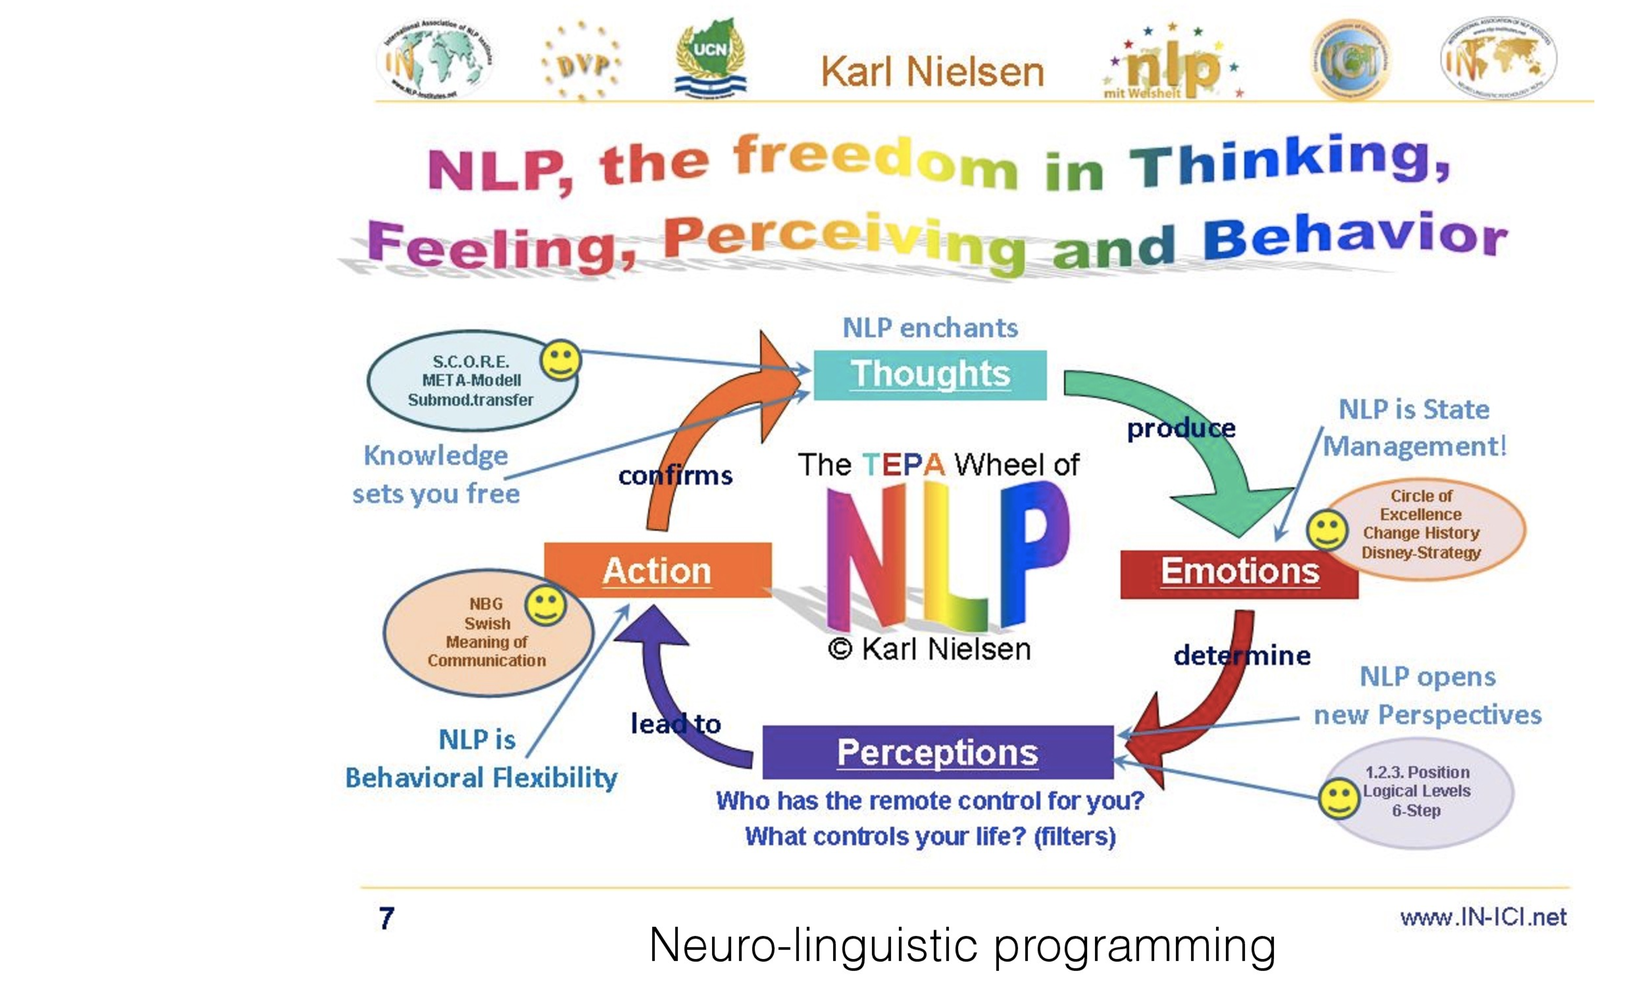
\includegraphics[width=0.83\paperwidth]{nlp1.png}}
	\begin{frame}
\end{frame}
}


{
	\usebackgroundtemplate{ 
		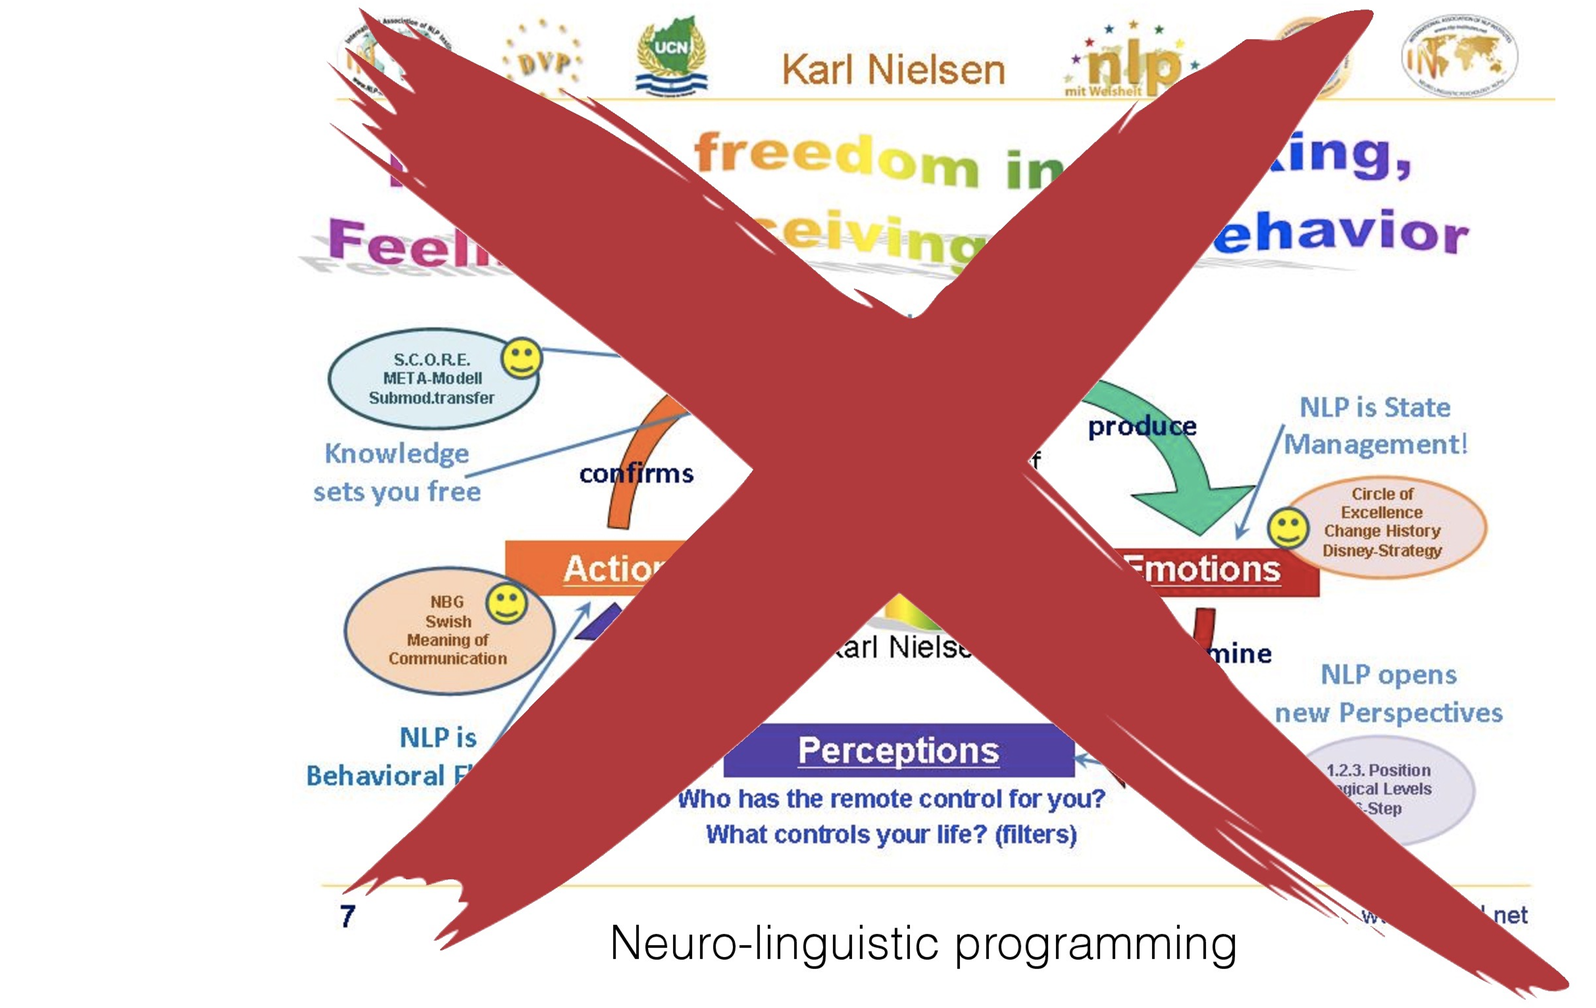
\includegraphics[width=0.83\paperwidth]{nlp2.png}}
	\begin{frame}
\end{frame}
}


\begin{frame}
\begin{center}
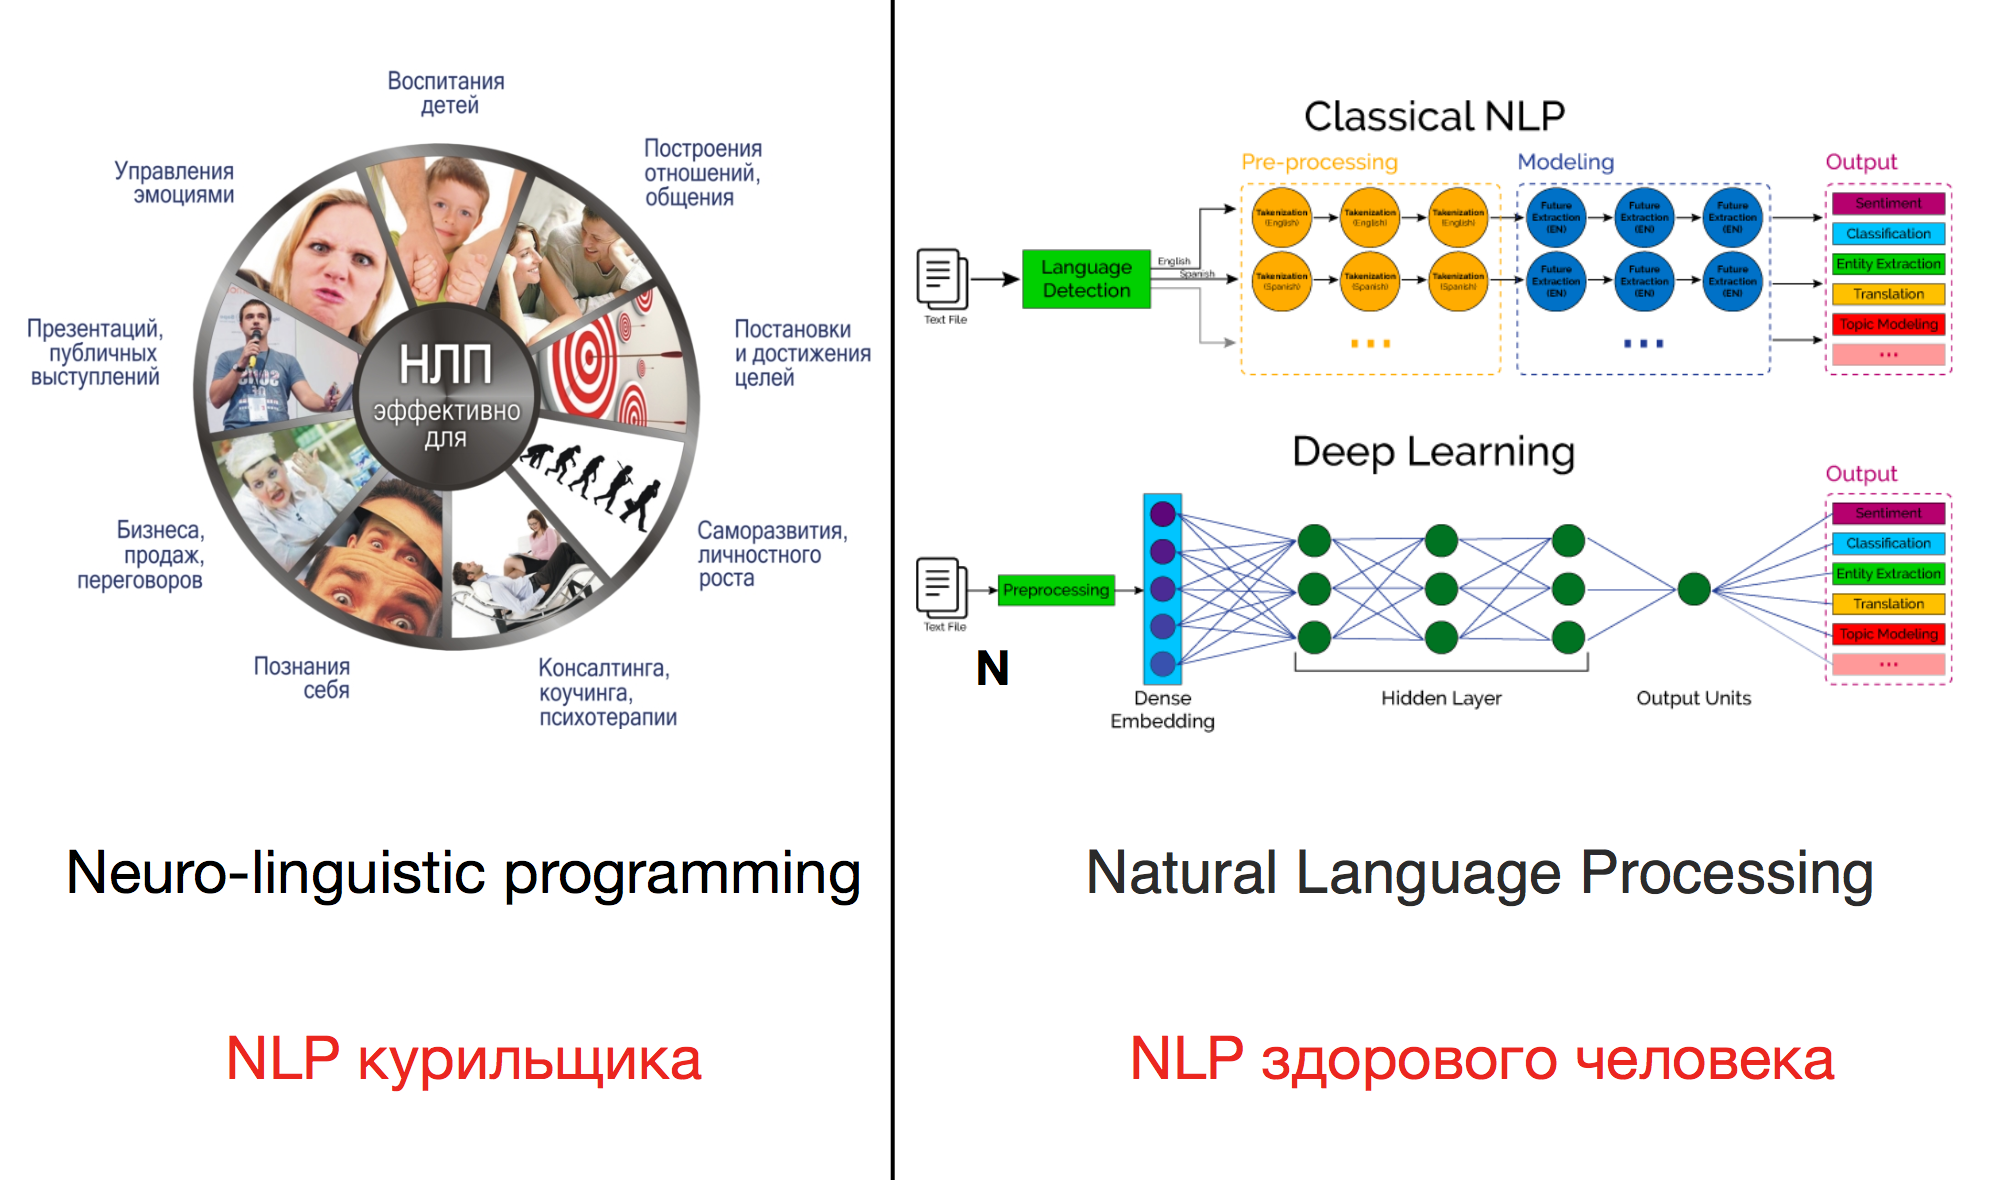
\includegraphics[width=0.8\paperwidth]{nlp5.png}
\end{center}
\end{frame}


\begin{frame}{Модели на текстах }
\begin{center}
	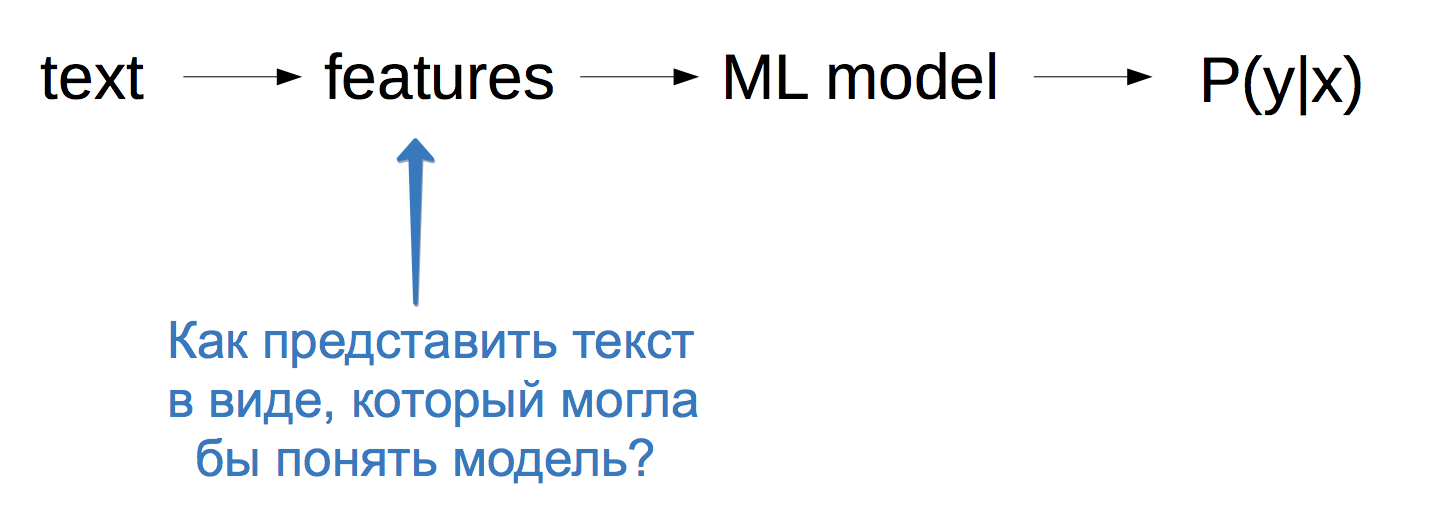
\includegraphics[width=.8\linewidth]{text1.png}
\end{center}
\end{frame} 


\begin{frame}
\begin{center}
	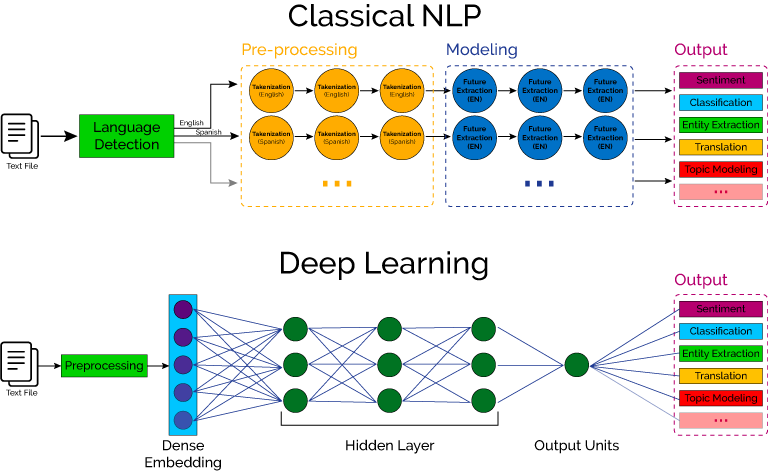
\includegraphics[width=0.8\paperwidth]{nn_vs_class.png}
\end{center}
\vfill
\footnotesize  {\color{blue} \url{https://www.nsuchaud.fr/2018/03/difference-between-classical-nlp-deep-learning-nlp/}}
\end{frame}


\begin{frame}{Что такое текст?}
\begin{columns}
\begin{column}{.48\linewidth}
	
\includegraphics[scale=0.3]{bender.png}
\end{column}

	\begin{column}{.48\linewidth}
\begin{wideitemize} 
	\item  Текст (документ) —  это последовательность токенов (слов)
	\item  Токен (слово) —  это последовательность символов
\end{wideitemize}
	\end{column}	
\end{columns}
\end{frame} 


\begin{frame}{One-Hot Encoding}
\begin{center}
	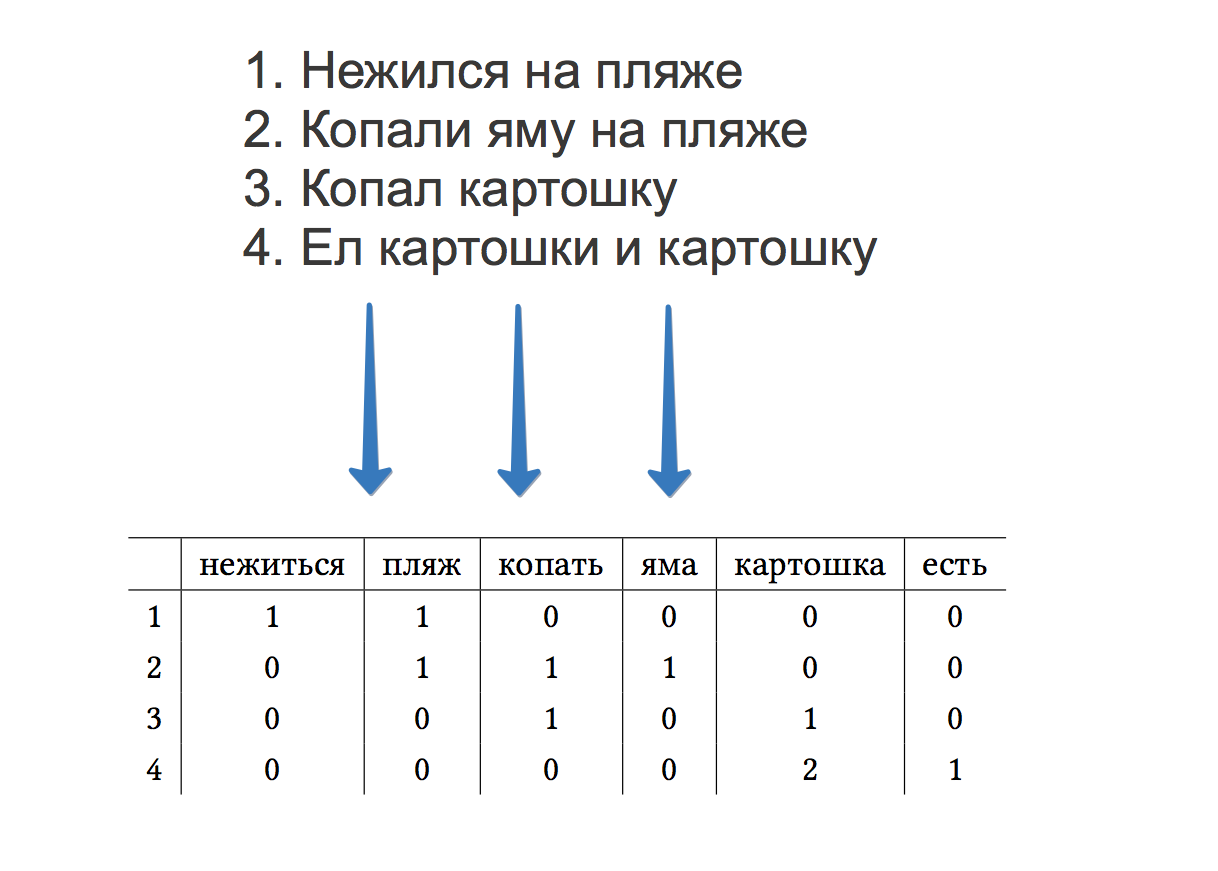
\includegraphics[width=.7\linewidth]{text.png}
\end{center}
\end{frame} 


\begin{frame}{One-Hot Encoding}
\begin{wideitemize} 
	\item  В словаре много слов, у нас будет слишком много признаков
	\item  В векторе нет никакой информации о смысле слова
	\item  Семантически похожие тексты могут иметь очень разные представления
	\item  Непонятно, что делать, если в тексте появляется какое-то новое слово
\end{wideitemize}
\end{frame} 


\begin{frame}{Гипотеза мешка слов}
	\begin{wideitemize} 
		\item \textbf{Гипотеза мешка слов:} нам плевать на взаимное расположение слов. Порядок слов в предложении никак не сказывается на его смысле. 	{\color{red}  Следуя гипотезе, мы теряем часть информации.}
		
		\item Рассматриваем каждое слово, как переменную $\Rightarrow$ большое пространство признаков. Нужно его урезать $\Rightarrow$ 	{\color{red}  Теряем ещё информацию.}
		
		\item Хотим маленькое пространство признаков и много информации в нём!
	\end{wideitemize}
\end{frame} 


\begin{frame}{Анализ текстов в одном слайде}
\begin{center}
	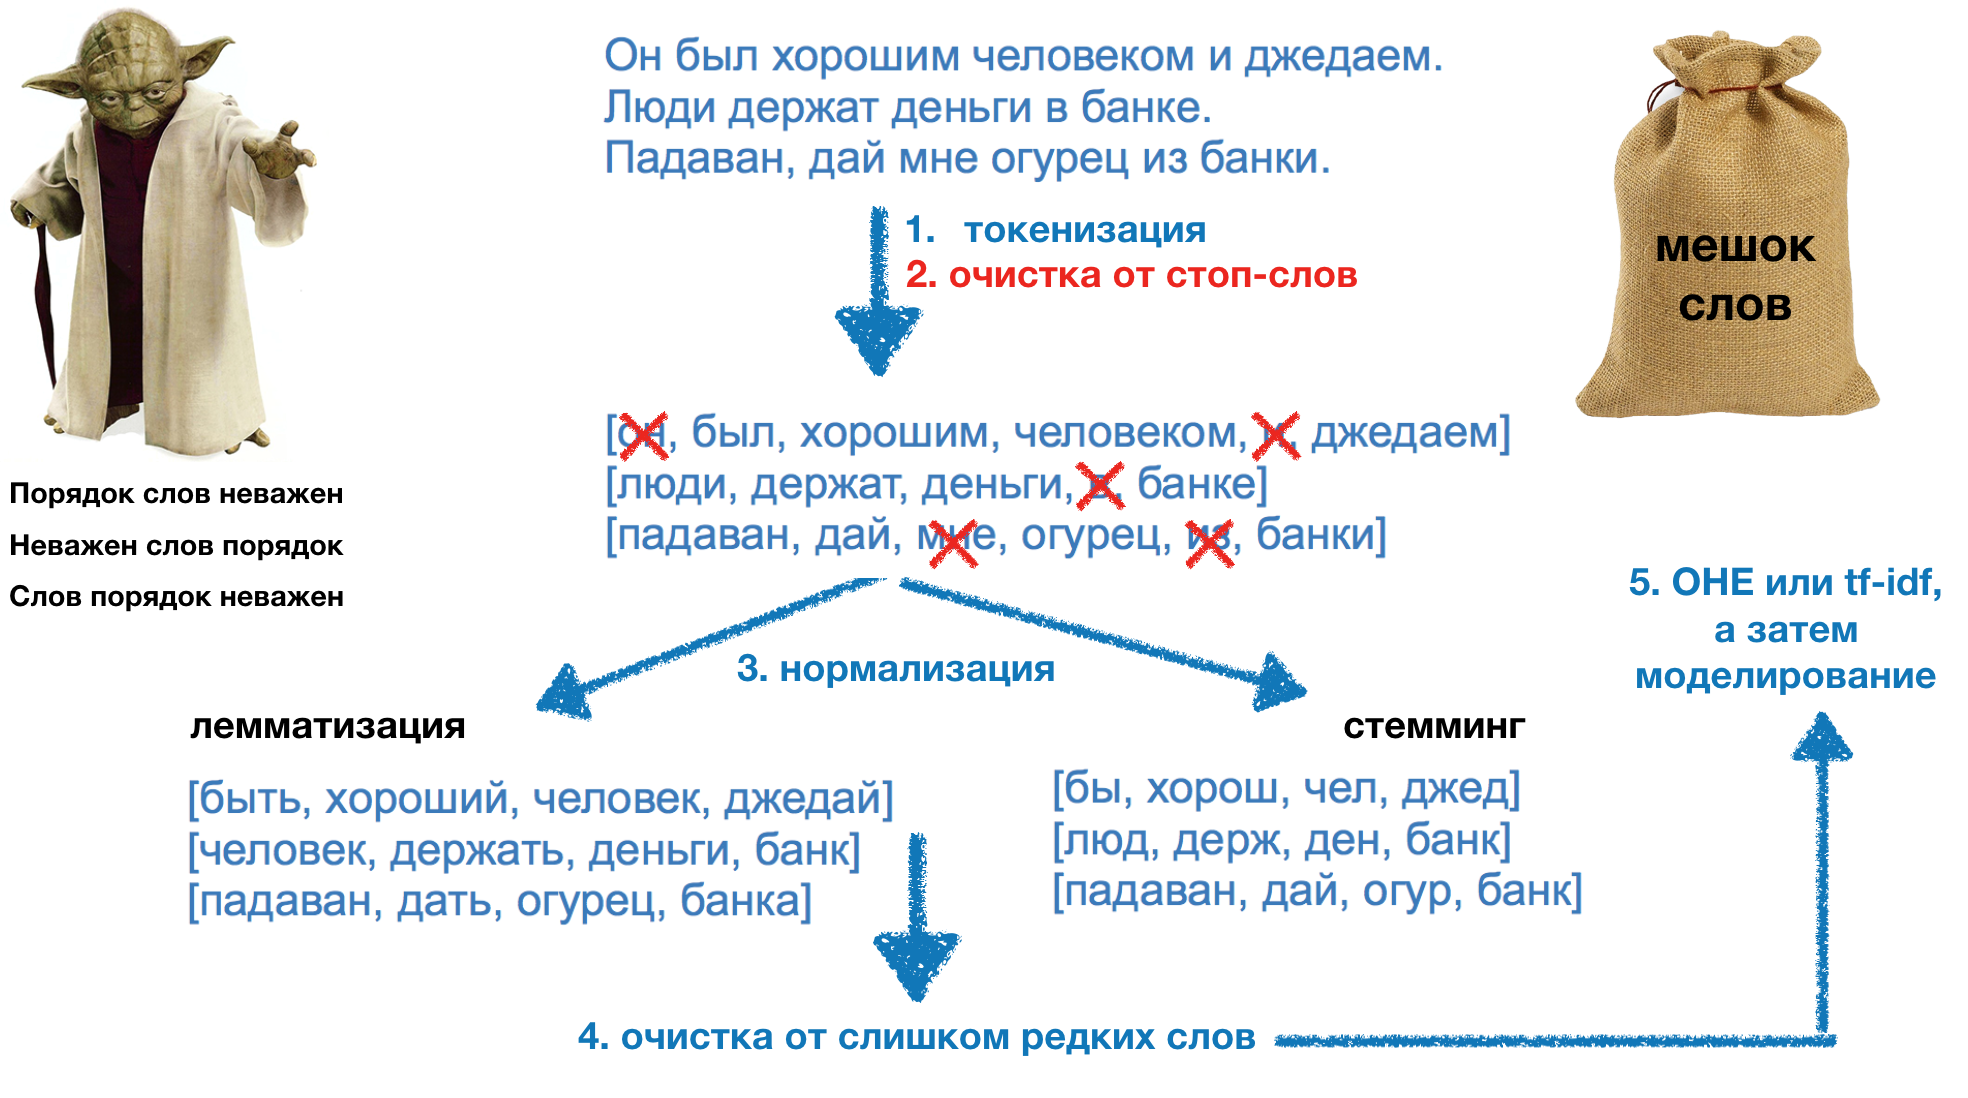
\includegraphics[width=.95\linewidth]{classic_text.png}
\end{center}
\end{frame} 


\begin{frame}{Tf-idf}
	\begin{wideitemize} 
		\item  \alert{tf (term frequency):} нормализация матрицы по строкам
		
		\item Если слово встречается в документе часто, но оно не стоп-слово, оно важное
		
		\item  Способы посчитать: 
		\begin{itemize}
			\item  частота слова 
			
			\item  булева частота слова (0 или 1)
			
			\item  log(частота)
			
			\item  любой свой способ
		\end{itemize}
	\end{wideitemize}
\end{frame} 


\begin{frame}{Tf-idf}
	\begin{wideitemize} 
		\item  \alert{idf (inverse document frequency):} нормализация матрицы по столбцам
		
		\item Слово встретилось только в этом документе, а в других нет, значит оно важное и описывает природу этого документа
		
		\item  Способы посчитать: 
		\begin{itemize}
			\item  $idf = 1$
			
			\item  $idf = log  \frac{N}{n_t}$
			
			\item  $idf = log \left(1 +  \frac{N}{n_t} \right)$
			
			\item  любой свой способ
		\end{itemize}
	\end{wideitemize}
\end{frame} 


\begin{frame}{Tf-Idf Encoding}
	\begin{center}
		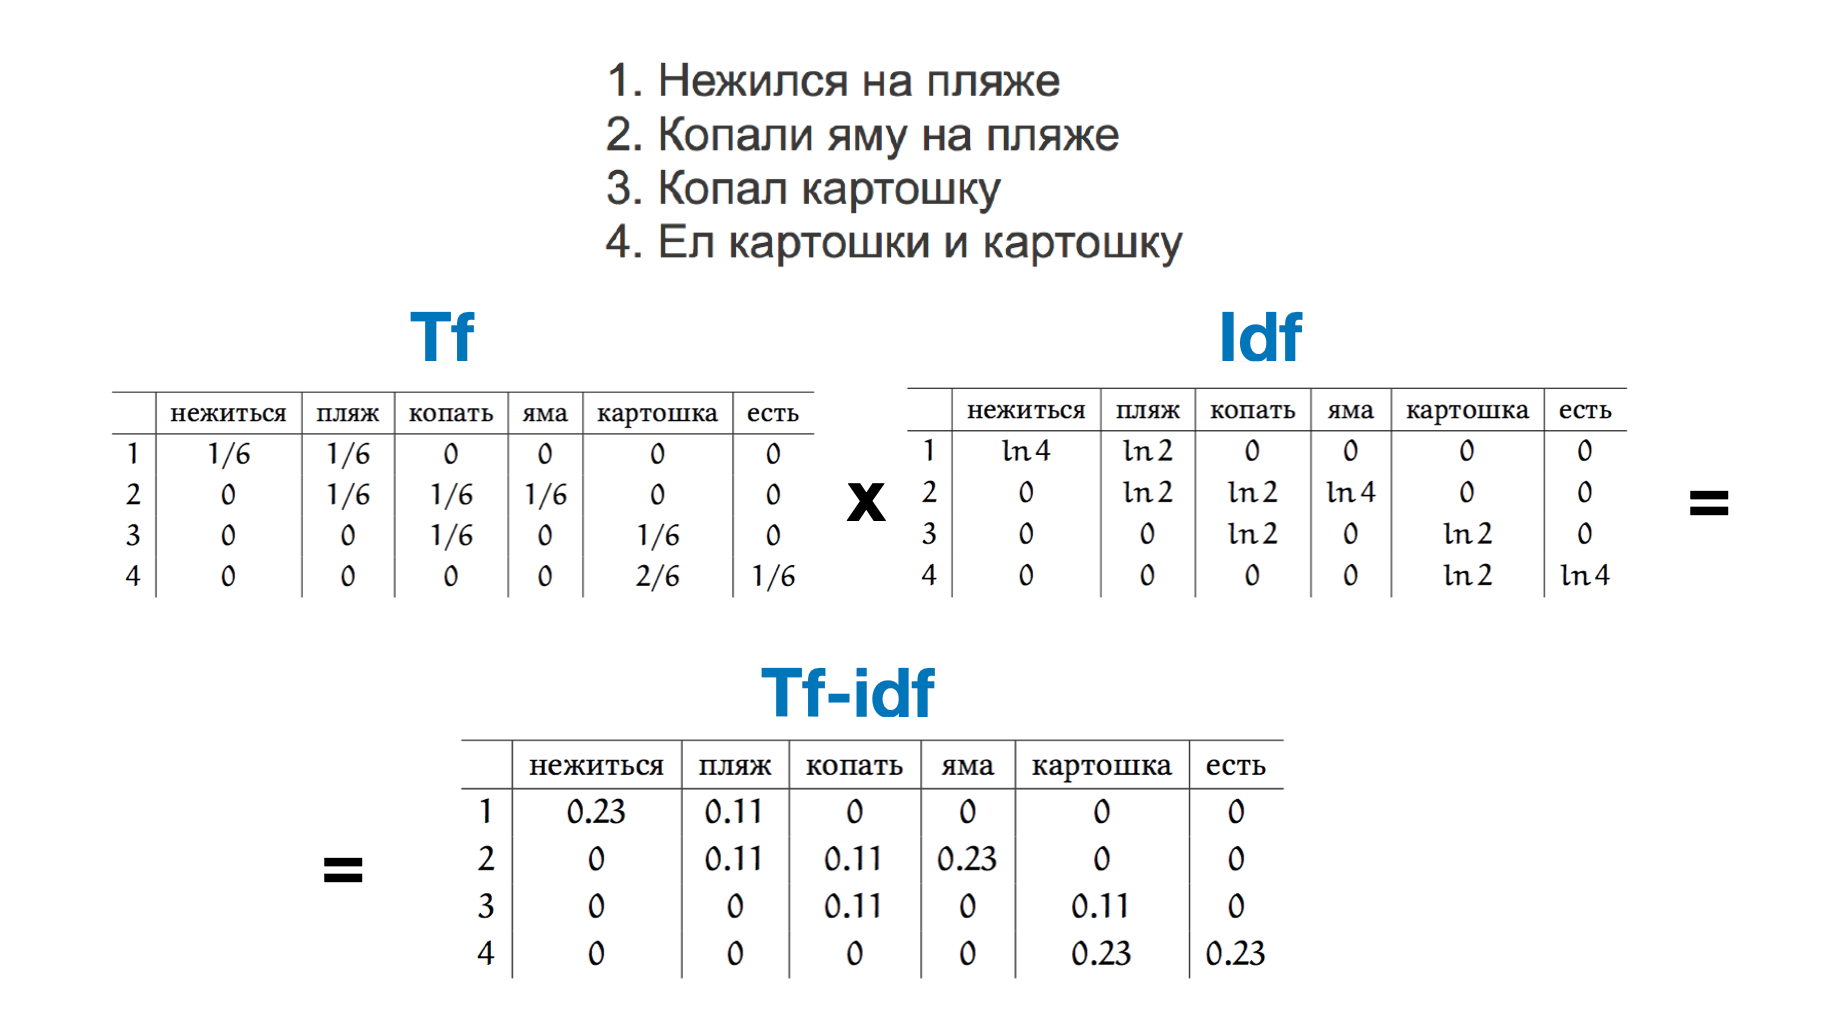
\includegraphics[width=.9\linewidth]{tf-idf.png}
	\end{center}
\end{frame} 


\begin{frame}{Tf-Idf Encoding}
	\begin{wideitemize} 
		\item  выбирая пороговые значения tf и idf можем решать какое число фичей взять в модель
		\item  idf убивает стоп-слова из-за того, что они встречаются почти в каждом документе
		\item  tf убивает редкие слова 
	\end{wideitemize}
\end{frame} 


\begin{frame}[shrink=10]{Какую модель учить?}
	
	\begin{wideitemize} 
		\item  Случайный лес жадно строит глубокие деревья минимизируя локальную ошибку вместо глобальной до тех пор, пока в листе не будет мало объектов. В нашей ситуации деревья будут очень глубокими $\Rightarrow$ \alert{долгий перебор}
		
		\item Текст хорошо описывается только с помощью совместного использования множества регрессоров. Лес требует очень большого числа деревьев для поиска закономерностей между разнесёнными по тексту словами. \alert{Чем больше деревьев, тем выше будет шум и сигнал затеряется.}
		
		\item Бустинг строит маленькие деревья. Каждое учит небольшое подмножество признаков. Целевая переменная объясняется комбинацией большого набора признаков  $\Rightarrow$ \alert{приходится использовать много деревьев, сигнал рассеивается.}
		
		\item  \alert{Логистическая регрессия отлично  подойдёт}
	\end{wideitemize}
\end{frame} 


\begin{frame}{Как сделать модель лучше?}
	\begin{center}
		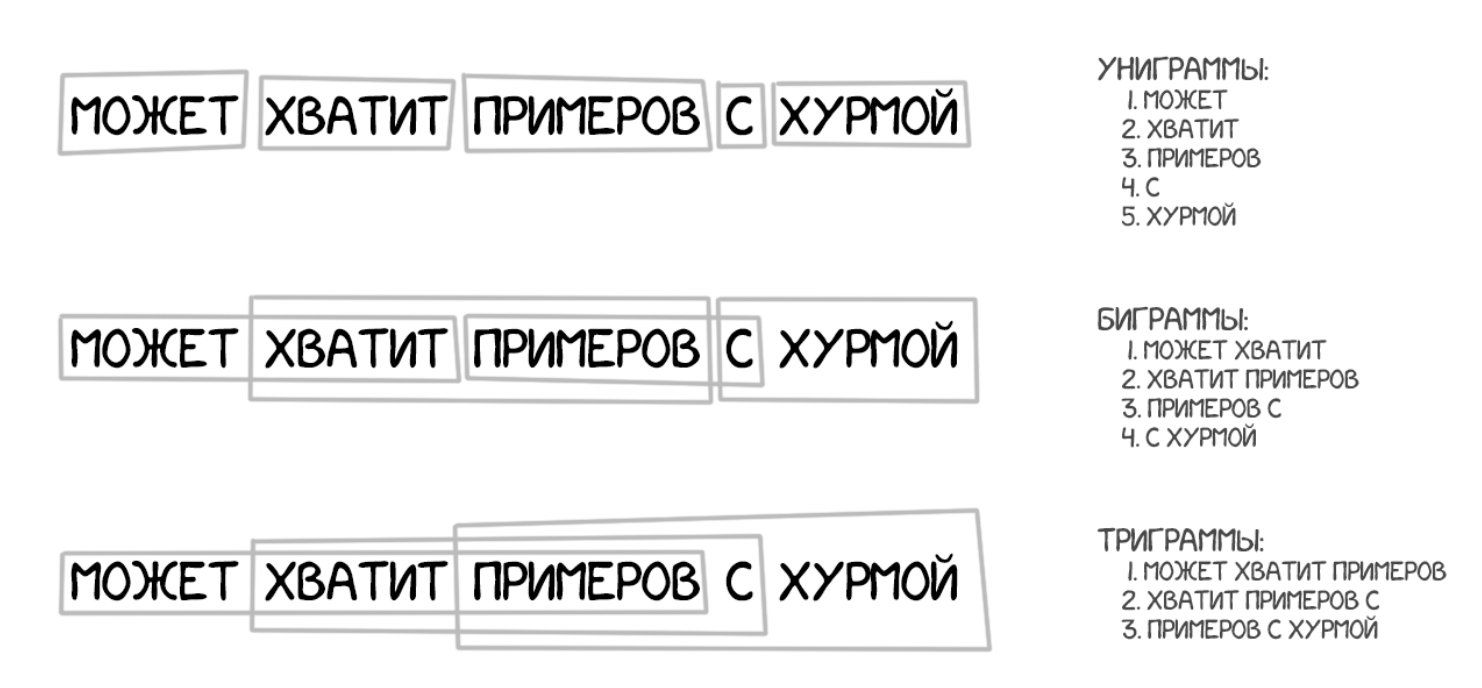
\includegraphics[width=.65\linewidth]{hurma.png}
	\end{center}
	\begin{itemize} 
		\item  Сейчас мы используем слова как фичи
		\item Почему бы не использовать пары из слов? 
		\item В общем виде n-граммы - последовательности из n слов
		\item Словарь разрастётся, но результат, возможно, улучшится
	\end{itemize}
\vfill
\footnotesize  {\color{blue} \url{https://vas3k.ru/blog/machine_translation/}}
\end{frame} 



\begin{frame}{Дистрибутивная гипотеза}
	\begin{wideitemize} 
		\item \textbf{Дистрибутивная гипотеза:} слова с похожим смыслом будут встречаться в похожих контекстах.
		\item Мы можем попытаться заложить в векторное представление слова информацию о его контексте
		\item Есть разные подходы: count-based и \alert{prediction-based,} мы поговорим о втором
	\end{wideitemize}
\end{frame} 


\begin{transitionframe}
	\begin{center}
		\Huge  Из слов в вектора и обратно
	\end{center}
	\centering 
\includegraphics[scale = 0.15]{bilbo.png}
\end{transitionframe}



\begin{frame}{Words embeddings}
\begin{wideitemize} 
	\item \textbf{Наша цель:}  хотим научить компьютер понимать слова
	\item Идея! Давайте превратим наши слова в вектора размера $d$
	\item На вектора понакладываем хотелок! 
\end{wideitemize} 
\begin{center}
	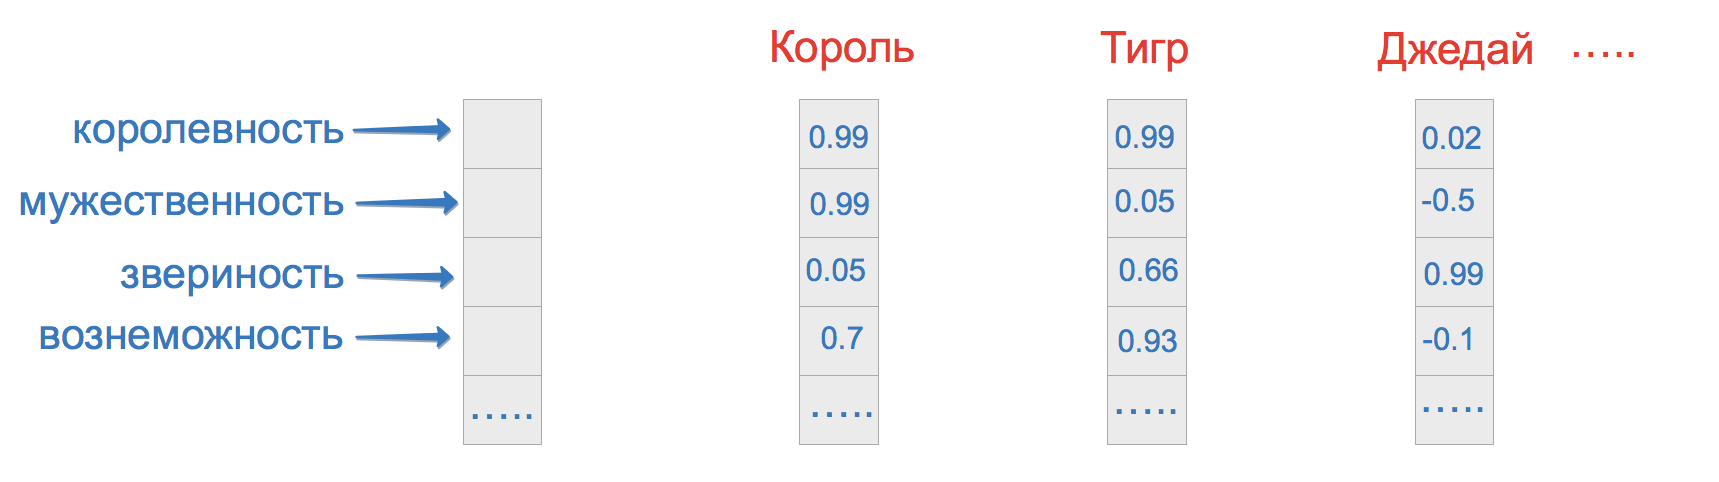
\includegraphics[width=.95\linewidth]{vectors.png}
\end{center}
\end{frame} 


\begin{frame}{Хотелка первая}
\begin{itemize} 
\item Хотим, чтобы модель улавливала семантические свойства слов
\end{itemize} 


\begin{center}
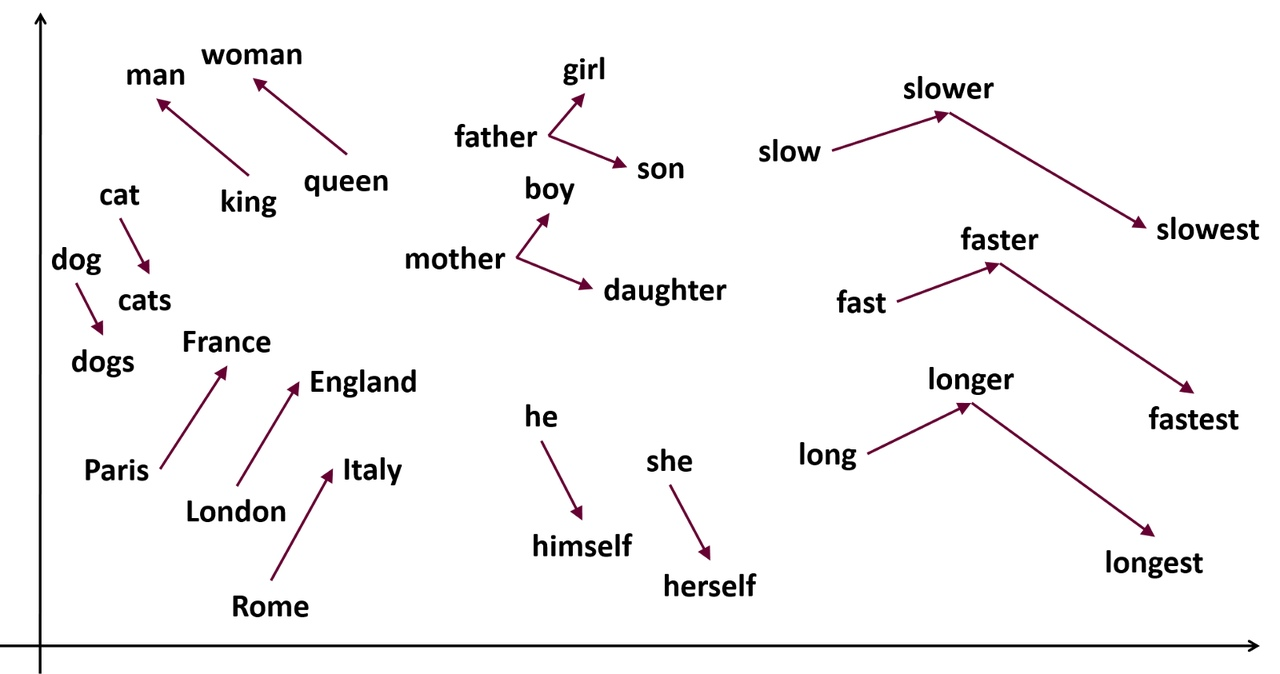
\includegraphics[width=.8\linewidth]{w2v_sim.jpg}
\end{center}
\end{frame} 


\begin{frame}{Хотелка вторая}
\begin{itemize} 
\item Модель понимала, где близкие по смыслу слова: кот, котёнок, кошка, тигр, лев, ...	
\end{itemize} 


\begin{center}
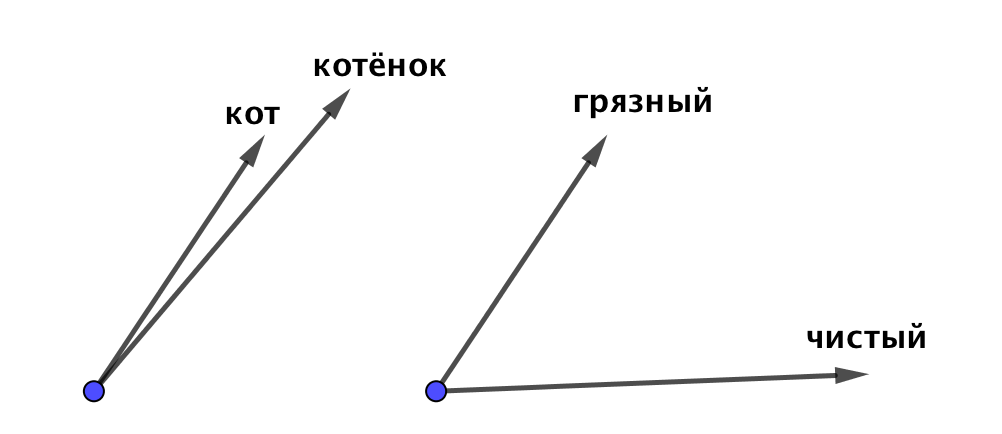
\includegraphics[width=.7\linewidth]{w2v_dist.png}
\end{center}
\end{frame} 


\begin{frame}{Хотелка третья}
\begin{itemize} 
\item Арифметика! 
\end{itemize} 

\begin{center}
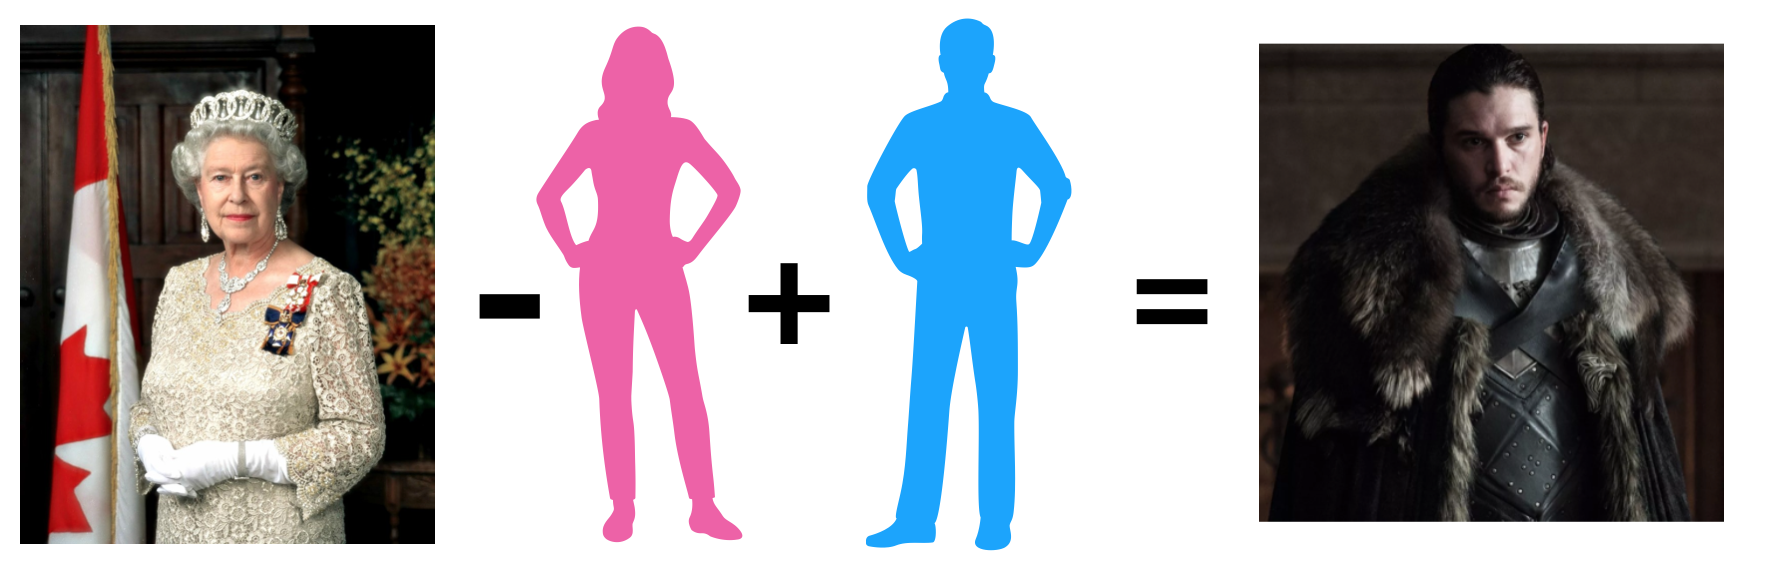
\includegraphics[width=.8\linewidth]{w2v_arith.png}
\end{center}
\end{frame} 


\begin{frame}{Томаш Миколов}
		\begin{columns}[T] 
				\begin{column}{.4\textwidth}
						\begin{wideitemize} 
						\item \alert{Звучит как магия, но правда работает}
						
						\item  В 2013 году модель предложена чешским аспирантом  Томашем Миколовым
						
						\item После работал в Google, сейчас ушёл в Facebook  
						\end{wideitemize} 
				\end{column}%
				\hfill%
				\begin{column}{.6\textwidth}
						\begin{center}
						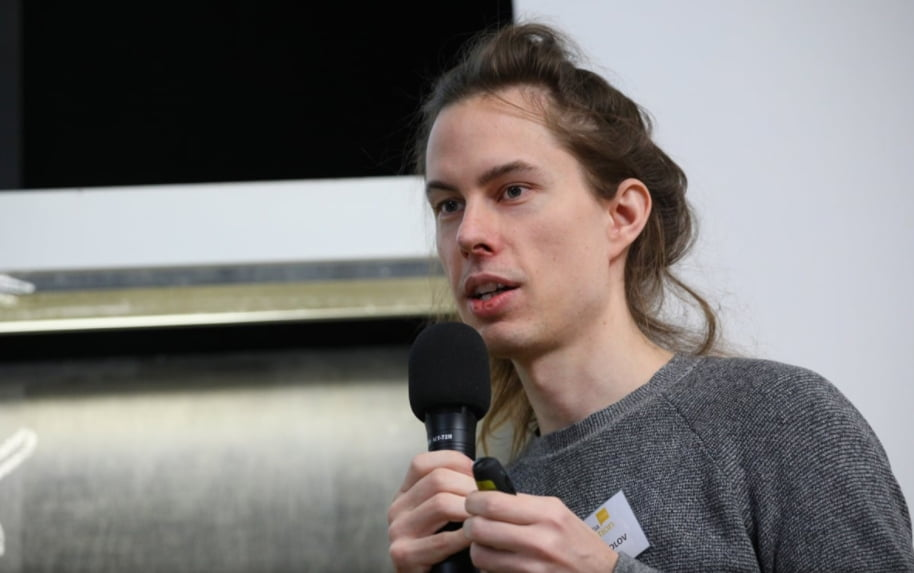
\includegraphics[width=.99\linewidth]{tomas-mikolov.jpg}
						\end{center}
				\end{column}%
		\end{columns}
		\vfill
		\footnotesize  {\color{blue} \url{https://arxiv.org/abs/1301.3781}}
\end{frame}


\begin{frame}{Идея word2vec}
	\begin{wideitemize} 
		\item \textbf{Основная идея:} мы хотим упаковать информацию о контексте слов в вектора
		 
		\item \textbf{Как это сделать:} будем обучать вектора, пытаясь предсказать контекст, в котором встречается слово (skip-gram)   
		
		\pause
		
		\item  \alert{CBOW (непрерывный мешок слов)} —  в нём мы по заданному контексту слова пытаемся предсказать слово
		
		\item \alert{Skip-gram} — по заданному слову пытаемся предсказать его контекст 
	\end{wideitemize}
\end{frame} 


\begin{frame}{NLP course for you}
	\begin{center}
		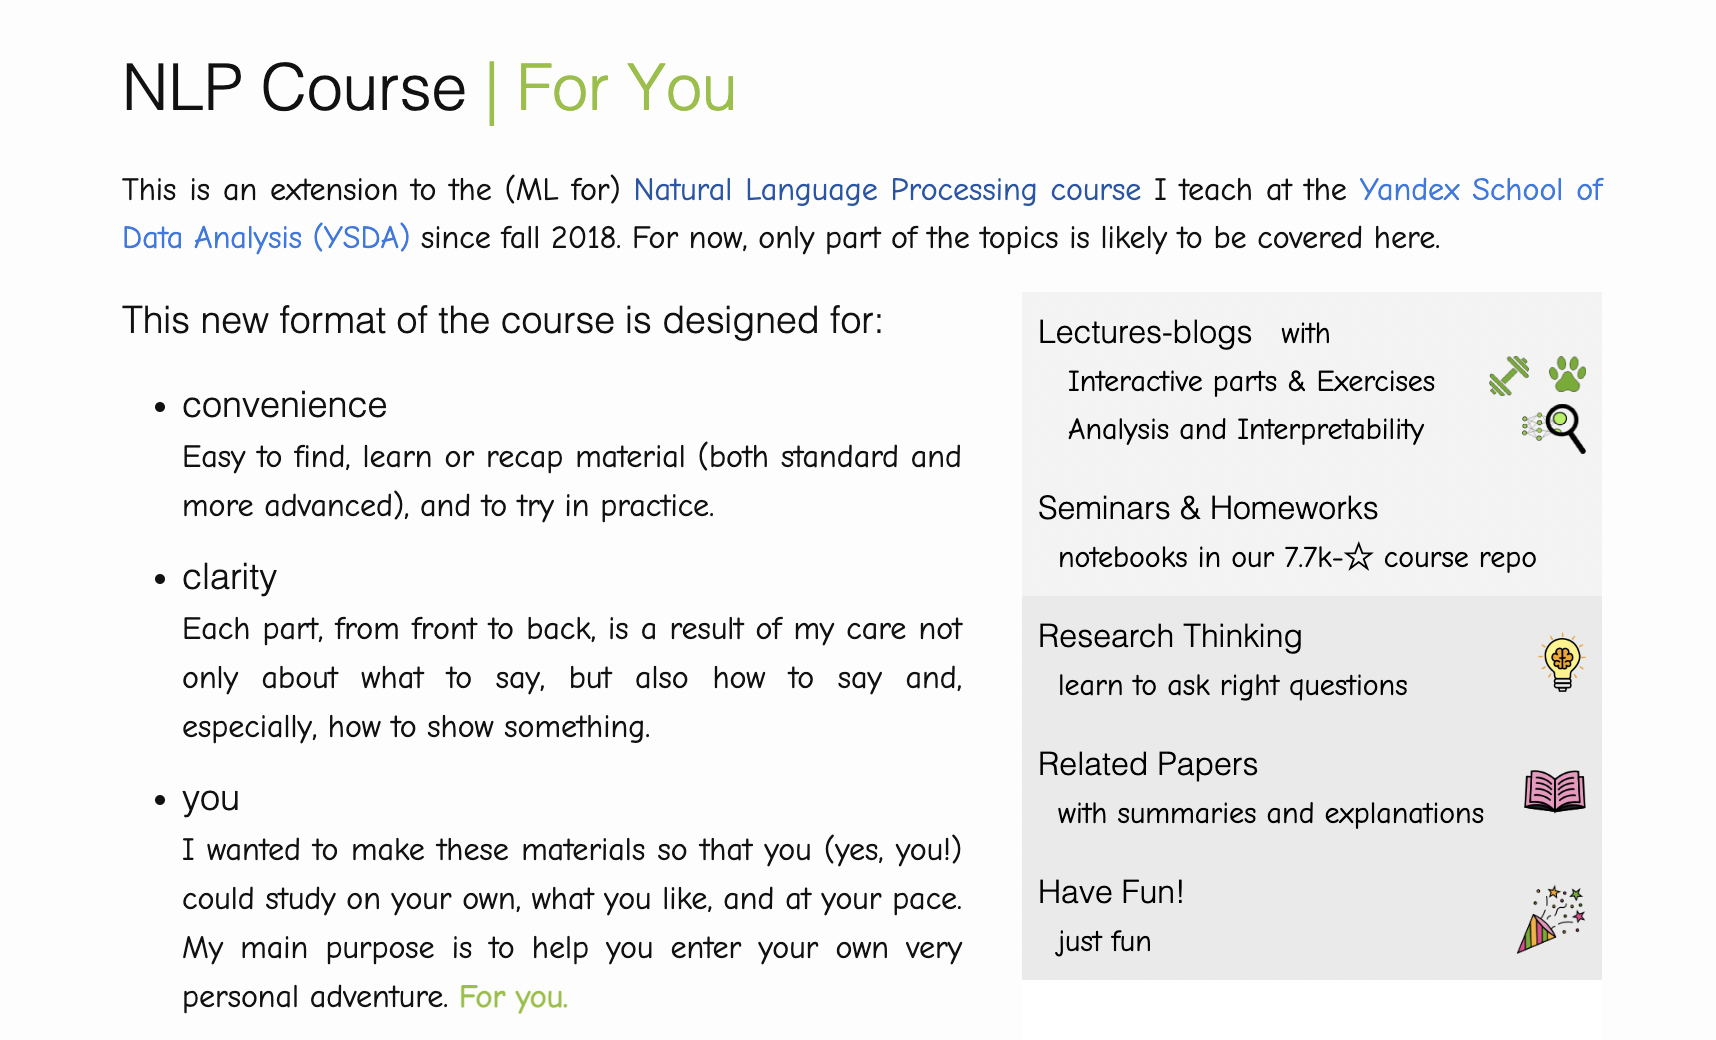
\includegraphics[width=.75\linewidth]{nlp_for_you.png}
	\end{center}
\vfill
\footnotesize  {\color{blue} \url{https://lena-voita.github.io/nlp_course/word_embeddings.html}}
\end{frame} 


\begin{frame}{w2v верхнеуровнево}	
		\begin{center}
			\begin{tikzpicture}	
				 \only<1>{\draw (0,0) node { \large ... I saw a cute grey cat playing in the garden ... };}
				 
				 \only<2-5>{
				 	\draw (0,0) node { \large ... $\underset{\small w_{t-2}}{\hbox{ \higgray{I}}}$ $\underset{\small w_{t-1}}{\hbox{\higgray{saw}}}$ $\underset{\small \color{green} w_{t}}{\hbox{\higgreen{a}}}$  $\underset{\small w_{t+1}}{\hbox{\higgray{ cute}}}$  $\underset{\small w_{t+2}}{\hbox{\higgray{grey}}}$  cat playing in the garden ... };
			 	}
		 	
		 		\only<3-5>{
		 		 \draw (-5,-1.5) node {\footnotesize \color{gray} context \\ \footnotesize \color{gray}  words };
		 		  \draw (-1,-1.5) node {\footnotesize \color{gray} context \\ \footnotesize \color{gray} words };
		 		  \draw (-3,-1.5) node {\footnotesize \color{green} central \\ \footnotesize  \color{green}  word };
		 	}
		 
		 	  \only<4-5>{ 
		 	  	 \draw (-6, 1) node {\scriptsize     $P(w_{t-2} \mid \color{green}{w_t} )$ };
		 	  	 \draw (-4, 1) node {\scriptsize	  $P(w_{t-1} \mid \color{green}{w_t})$ }; 	 
		 	  	 \draw (-2, 1) node {\scriptsize	  $P(w_{t+1} \mid \color{green}{w_t})$ }; 
		 	  	  \draw (0, 1) node {\scriptsize	  $P(w_{t+2} \mid \color{green}{w_t})$ }; 	 	 
		  	}
		  
		   \only<6>{ 
			   	\draw (0,0) node { \large ... I $\underset{\small w_{t-2}}{\hbox{ \higgray{saw}}}$ $\underset{\small w_{t-1}}{\hbox{\higgray{a}}}$ $\underset{\small \color{green} w_{t}}{\hbox{\higgreen{cute}}}$  $\underset{\small w_{t+1}}{\hbox{\higgray{ grey}}}$  $\underset{\small w_{t+2}}{\hbox{\higgray{cat}}}$ playing in the garden ... };
			   	
			   	 \draw (-4.5,-1.5) node {\footnotesize \color{gray} context \\ \footnotesize \color{gray}  words };
			   	\draw (-0.5,-1.5) node {\footnotesize \color{gray} context \\ \footnotesize \color{gray} words };
			   	\draw (-2.5,-1.5) node {\footnotesize \color{green} central \\ \footnotesize  \color{green}  word };
		   	
		   	 	 \draw (-5, 1) node {\scriptsize     $P(w_{t-2} \mid \color{green}{w_t} )$ };
		   		 \draw (-3, 1) node {\scriptsize	  $P(w_{t-1} \mid \color{green}{w_t})$ }; 	 
		   		 \draw (-1, 1) node {\scriptsize	  $P(w_{t+1} \mid \color{green}{w_t})$ }; 
		   		 \draw (1, 1) node {\scriptsize	  $P(w_{t+2} \mid \color{green}{w_t})$ }; 	 
		   }
		
		   \only<7>{ 
				\draw (0,0) node { \large ... I saw $\underset{\small w_{t-2}}{\hbox{ \higgray{a}}}$ $\underset{\small w_{t-1}}{\hbox{\higgray{cute}}}$ $\underset{\small \color{green} w_{t}}{\hbox{\higgreen{grey}}}$  $\underset{\small w_{t+1}}{\hbox{\higgray{cat}}}$  $\underset{\small w_{t+2}}{\hbox{\higgray{playing}}}$  in the garden ... };
				
				\draw (-3.5,-1.5) node {\footnotesize \color{gray} context \\ \footnotesize \color{gray}  words };
				\draw (0.5,-1.5) node {\footnotesize \color{gray} context \\ \footnotesize \color{gray} words };
				\draw (-1.5,-1.5) node {\footnotesize \color{green} central \\ \footnotesize  \color{green}  word };
				
				\draw (-4, 1) node {\scriptsize     $P(w_{t-2} \mid \color{green}{w_t} )$ };
				\draw (-2, 1) node {\scriptsize	  $P(w_{t-1} \mid \color{green}{w_t})$ }; 	 
				\draw (0, 1) node {\scriptsize	  $P(w_{t+1} \mid \color{green}{w_t})$ }; 
				\draw (2, 1) node {\scriptsize	  $P(w_{t+2} \mid \color{green}{w_t})$ }; 	 
			}
		
		   \only<8>{ 
				\draw (0,0) node { \large ... I saw a $\underset{\small w_{t-2}}{\hbox{ \higgray{cute}}}$ $\underset{\small w_{t-1}}{\hbox{\higgray{grey}}}$ $\underset{\small \color{green} w_{t}}{\hbox{\higgreen{cat}}}$  $\underset{\small w_{t+1}}{\hbox{\higgray{playing}}}$  $\underset{\small w_{t+2}}{\hbox{\higgray{in}}}$  the garden ... };
				
				\draw (-2.5,-1.5) node {\footnotesize \color{gray} context \\ \footnotesize \color{gray}  words };
				\draw (1.5, -1.5) node {\footnotesize \color{gray} context \\ \footnotesize \color{gray} words };
				\draw (-0.5,-1.5) node {\footnotesize \color{green} central \\ \footnotesize  \color{green}  word };
				
				\draw (-3, 1) node {\scriptsize     $P(w_{t-2} \mid \color{green}{w_t} )$ };
				\draw (-1, 1) node {\scriptsize	  $P(w_{t-1} \mid \color{green}{w_t})$ }; 	 
				\draw (1, 1) node {\scriptsize	  $P(w_{t+1} \mid \color{green}{w_t})$ }; 
				\draw (3, 1) node {\scriptsize	  $P(w_{t+2} \mid \color{green}{w_t})$ }; 	 
			}
			\end{tikzpicture}
		\end{center}
				
		\begin{itemize}
			\item  Собрали большой корпус из текстов
			 \only<2->{\item Идём по тексту скользящим окном}
			\only<4->{\item  Расчитаем вероятность встретить контекст при условии что центральное слово фиксировано}
			\only<5->{\item  Вектора $w_i$ должны максимизировать вероятности}
		\end{itemize}
\end{frame} 


\begin{frame}{Правдоподобие модели}
	\begin{wideitemize} 
			\item  word2vec пытается максимизировать правдоподобие текстов:
			
				\[ 
					L(\theta)  = \prod_{t = 1}^T \prod_{ \substack{ j \ne 0 \\ -m \le j \le m}} P(w_{t + j} \mid w_t, \theta)
				\]
				
			\item Чтобы получить функцию потерь, прологарифмируем и умножим на $-1$:
			
				\[
					Loss = J(\theta) = - \frac{1}{T} \log L(\theta)  =  - \frac{1}{T} \sum_{t=1}^T  \sum_{ \substack{ j \ne 0 \\ -m \le j \le m}} log P(w_{t + j} \mid w_t, \theta)
				\]
				
			\item \alert{Осталось договориться как мы будем считать вероятность} 
		
		\end{wideitemize} 
\end{frame} 



\begin{frame}{Как считать вероятность?} 
	
	\mbox{  }
	
	Для каждого слова $w$ будем обучать два вектора:
	
	\mbox{  }
	
	\begin{columns}[T] 
			\begin{column}{.4\textwidth}					
					\begin{wideitemize} 
						\item  $v_{w}$ — когда это слово центральное
						\item  $u_{w}$ — когда это слово входит в контекст
						\item  после обучения обычно используют только вектора слов, $V$
						\item  про вектора контекста, $U$, забывают
					\end{wideitemize} 	

				\end{column}%
			\hfill%
			\begin{column}{.6\textwidth}
					\begin{center}
						\begin{tikzpicture}	
							\definecolor{zzttqq}{rgb}{0.85,0.42,0.08}
							\definecolor{qqqqff}{rgb}{0,0.4,0.7}
							\definecolor{qqwuqq}{rgb}{0,0.5,0}			
							
							\draw[line width=2.pt,color=qqwuqq] (-3.,5.) -- (-3.,2.) -- (-1.,2.) -- (-1.,5.) -- cycle;
							\fill[line width=2.pt,color=qqwuqq, fill=qqwuqq, fill opacity=0.3] (-3.,4.) -- (-1.,4.) -- (-1.,3.8) -- (-3.,3.8) -- cycle;
							
							\draw[line width=2.pt,color=qqqqff] (0.,5.) -- (0.,2.) -- (2.,2.) -- (2.,5.) -- cycle;
							\fill[line width=2.pt,color=qqqqff, fill=qqqqff, fill opacity=0.3] (0.,4.3) -- (2.,4.3) -- (2.,4.1) -- (0.,4.1) -- cycle;
							
							\draw (-2,  5.3) node{\color{qqwuqq} центральные \\ \color{qqwuqq}  слова };
							\draw (1.1, 5.2) node{ \color{qqqqff} контекст };
							
							\draw (-4,4.2) node[anchor=north west] { { \color{qqwuqq} cat} };
							\draw (-2.6,3) node[anchor=north west] {  { \color{qqwuqq} \Large $V$}  };
							\draw (0.4,3) node[anchor=north west] { { \color{qqqqff} \Large $U$} };
							
							\draw[line width=1.pt, ->] (2.3, 2) -- (2.3, 5);
							\draw[line width=1.pt, ->] (2.3, 5) -- (2.3, 2);
							\draw (3.2, 3) node{размер \\ словаря};
							
							\draw[line width=1.pt, color=qqwuqq, ->] (-3, 1.7) -- (-1, 1.7);
							\draw[line width=1.pt, color=qqwuqq, ->]  (-1, 1.7) --(-3, 1.7);
							\draw (-2, 0.8) node{\color{qqwuqq} \small размер \\ \color{qqwuqq} \small вектора};

							\draw[line width=1.pt, color=qqqqff, ->] (0, 1.7) -- (2, 1.7);
							\draw[line width=1.pt, color=qqqqff, ->]  (2, 1.7) --(0, 1.7);
							\draw (1, 0.8) node{\color{qqqqff} \small размер \\ \color{qqqqff} \small вектора};							
						\end{tikzpicture}
					\end{center}
				\end{column}%
		\end{columns}
\end{frame}


\begin{frame}{Как считать вероятность?} 

	\mbox{  }
	
	Для центрального слова {\color{green} $c$} и контекстного слова  {\color{gray} $o$} :
	
	\mbox{  }

	\[
		P({\color{gray} o} \mid {\color{green} c} ) = \frac{exp({\color{gray} u_o^T}  {\color{green} v_c)}}{\sum_{w \in V}  exp({\color{gray} u^T_w}  {\color{green} v_c} )}
	\] 
	
	\begin{wideitemize} 
		\item  обычный softmax
		\item  чем выше ${\color{gray} u_o^T}  {\color{green} v_c}$ тем больше вероятность встретить настоящее слово  ${\color{gray} o}$ контексте центрального {\color{green} $c$} 
        \item хотим, чтобы вероятности для пар слов, встречающихся в данных, были высокими, а для пар не встречающихся в данных низкими
	\end{wideitemize} 

\end{frame}


\begin{transitionframe}
	\begin{center}
			\Huge  Обучение модели
		\end{center}
 	\centering 
\includegraphics[scale = 0.15]{bilbo.png}
\end{transitionframe}



\begin{frame}{Один шаг обучения в деталях}
	
		\begin{center}
			\begin{tikzpicture}					
					\draw (0,0) node { \large ... I saw a $\underset{\small w_{t-2}}{\hbox{ \higgray{cute}}}$ $\underset{\small w_{t-1}}{\hbox{\higgray{grey}}}$ $\underset{\small \color{green} w_{t}}{\hbox{\higgreen{cat}}}$  $\underset{\small w_{t+1}}{\hbox{\higgray{playing}}}$  $\underset{\small w_{t+2}}{\hbox{\higgray{in}}}$  the garden ... };

					\draw (-2.5,-1.5) node {\footnotesize \color{gray} context \\ \footnotesize \color{gray}  words };
					\draw (1.5, -1.5) node {\footnotesize \color{gray} context \\ \footnotesize \color{gray} words };
					\draw (-0.5,-1.5) node {\footnotesize \color{green} central \\ \footnotesize  \color{green}  word };
					
					\draw (-3, 1) node {\scriptsize     $P(w_{t-2} \mid \color{green}{w_t} )$ };
					\draw (-1, 1) node {\scriptsize	  $P(w_{t-1} \mid \color{green}{w_t})$ }; 	 
					\draw (1, 1) node {\scriptsize	  $P(w_{t+1} \mid \color{green}{w_t})$ }; 
					\draw (3, 1) node {\scriptsize	  $P(w_{t+2} \mid \color{green}{w_t})$ }; 	 
			\end{tikzpicture}
		\end{center}
		
		\vfill 
		
		\only<1>{		
			\[
			Loss = J(\theta) = - \frac{1}{T} \log L(\theta)  =  - \frac{1}{T} \sum_{t=1}^T  \sum_{ \substack{ j \ne 0 \\ -m \le j \le m}} \log P( {\color{gray} w_{t + j}}  \mid  {\color{green} w_t}, \theta) 
			\]
			
			\[ \theta = \{U, V\} \]
		}
	
		\only<2>{			
			\[
			Loss = J(\theta) = - \frac{1}{T} \log L(\theta)  =  - \frac{1}{T} \sum_{t=1}^T  \sum_{ \substack{ j \ne 0 \\ -m \le j \le m}} J_{t,j} (\theta)
			\]
			
			$J_{t,j} (\theta)$ — потери для слова $j$ в окне $t$ 
		}
\end{frame}


\begin{frame}{Один шаг обучения в деталях}
	
\begin{center}
	\begin{tikzpicture}					
		\draw (0,0) node { \large ... I saw a $\underset{\small w_{t-2}}{\hbox{ \higgray{cute}}}$ $\underset{\small w_{t-1}}{\hbox{\higgray{grey}}}$ $\underset{\small \color{green} w_{t}}{\hbox{\higgreen{cat}}}$  $\underset{\small w_{t+1}}{\hbox{\higgray{playing}}}$  $\underset{\small w_{t+2}}{\hbox{\higgray{in}}}$  the garden ... };
		
		\draw (-2.5,-1.5) node {\footnotesize \color{gray} context \\ \footnotesize \color{gray}  words };
		\draw (1.5, -1.5) node {\footnotesize \color{gray} context \\ \footnotesize \color{gray} words };
		\draw (-0.5,-1.5) node {\footnotesize \color{green} central \\ \footnotesize  \color{green}  word };
		
		\draw (-3, 1) node {\scriptsize     $P(w_{t-2} \mid \color{green}{w_t} )$ };
		\draw (-1, 1) node {\scriptsize	  $P(w_{t-1} \mid \color{green}{w_t})$ }; 	 
		\draw (1, 1) node {\scriptsize	  $P(w_{t+1} \mid \color{green}{w_t})$ }; 
		\draw (3, 1) node {\scriptsize	  $P(w_{t+2} \mid \color{green}{w_t})$ }; 	 
	\end{tikzpicture}
\end{center}


	\begin{columns}[T] 
		\begin{column}{.5\textwidth}
			\vspace{1cm} 
			Потери на одном слове:
		{\small \[ 
			 - \log P({\color{blue} cute} \mid {\color{green} cat} ) = - \log \frac{ \exp({\color{blue}  u^T_{cute}} {\color{green}  v_{cat}} )}{\sum_w \exp({\color{blue}  u_w^T} {\color{green} v_{cat} }) }   
			\]}
		\end{column}%
		\hfill%
		\begin{column}{.5\textwidth}
			\begin{center}
				\begin{tikzpicture}	
					\definecolor{qqqqff}{rgb}{0,0.4,0.7}
						\draw[line width=1.5pt,color=green] (-3.,5.) -- (-3.,2.) -- (-1.,2.) -- (-1.,5.) -- cycle;
						\fill[line width=2.pt,color=green, fill=green, fill opacity=0.3] (-3.,4.) -- (-1.,4.) -- (-1.,3.8) -- (-3.,3.8) -- cycle;
						
						\draw[line width=1.5pt,color=qqqqff] (0.,5.) -- (0.,2.) -- (2.,2.) -- (2.,5.) -- cycle;
						\fill[line width=2.pt,color=qqqqff, fill=qqqqff, fill opacity=0.3] (0.,4.3) -- (2.,4.3) -- (2.,4.1) -- (0.,4.1) -- cycle;
						\fill[line width=2.pt,color=qqqqff, fill=qqqqff, fill opacity=0.3] (0.,4.8) -- (2.,4.8) -- (2.,4.6) -- (0.,4.6) -- cycle;
						\fill[line width=2.pt,color=qqqqff, fill=qqqqff, fill opacity=0.3] (0.,3) -- (2.,3) -- (2.,3.2) -- (0.,3.2) -- cycle;
						\fill[line width=2.pt,color=qqqqff, fill=qqqqff, fill opacity=0.3] (0.,3.7) -- (2.,3.7) -- (2.,3.5) -- (0.,3.5) -- cycle;
						
						\draw (-4,4.2) node[anchor=north west] { { \color{green} cat} };
						
						\draw (2, 4.6) node[anchor=north west] { { \color{qqqqff} cute} };
						\draw (2, 5.1) node[anchor=north west] { { \color{qqqqff} grey} };
						\draw (2, 3.9) node[anchor=north west] { { \color{qqqqff} playing} };
						\draw (2, 3.4) node[anchor=north west] { { \color{qqqqff} in} };
						
						\draw (-2.7,2) node[anchor=north west] {  { \color{green} \Large $V$}  };
						\draw (0.3,2) node[anchor=north west] { { \color{qqqqff} \Large $U$} };
				\end{tikzpicture}
			\end{center}
		\end{column}%
	\end{columns}
\end{frame}



\begin{frame}{Один шаг обучения в деталях}
	\definecolor{qqqqff}{rgb}{0,0.4,0.7}
	\definecolor{qqwuqq}{rgb}{0,0.5,0}
	
	 \[ 
	- \log P({\color{blue} cute} \mid {\color{green} cat} ) = - \log \frac{ \exp({\color{blue}  u^T_{cute}} {\color{green}  v_{cat}} )}{\sum_w \exp({\color{blue}  u_w^T} {\color{green} v_{cat} }) }   = - {\color{blue}  u^T_{cute}} {\color{green}  v_{cat}} +  \log \sum_w \exp({\color{blue}  u_w^T} {\color{green} v_{cat} })
	\]
	
	\pause 
	
	\vspace{0.5cm}

	\begin{columns}[T] 
	\begin{column}{.3\textwidth}
		\begin{center}
			\begin{tikzpicture}	
				\definecolor{qqqqff}{rgb}{0,0.4,0.7}
				\draw[line width=1.5pt,color=green] (-3.,5.) -- (-3.,2.) -- (-1.,2.) -- (-1.,5.) -- cycle;
				\fill[line width=2.pt,color=green, fill=green, fill opacity=0.3] (-3.,4.) -- (-1.,4.) -- (-1.,3.8) -- (-3.,3.8) -- cycle;
				
				\draw[line width=1.5pt,color=qqqqff] (0.,5.) -- (0.,2.) -- (2.,2.) -- (2.,5.) -- cycle;
				\fill[line width=2.pt,color=qqqqff, fill=qqqqff, fill opacity=0.3] (0.,4.3) -- (2.,4.3) -- (2.,4.1) -- (0.,4.1) -- cycle;
				
				\draw (-3.2, 4.5) node[anchor=north west] { { \color{green} cat} };
				
				\draw (-0.2, 4.85) node[anchor=north west] { { \color{qqqqff} cute} };
				
				\draw (-2.7,2) node[anchor=north west] {  { \color{green} \Large $V$}  };
				\draw (0.3,2) node[anchor=north west] { { \color{qqqqff} \Large $U$} };
			\end{tikzpicture}
		\end{center}
	\end{column}%
	\begin{column}{.7\textwidth}
		\begin{center}
			\begin{tikzpicture}	
					\draw (2, 5.3) node[anchor=north west] { $u_{w_1}^T {\color{qqwuqq} v_{cat}} $};
					\draw (2, 4.7) node[anchor=north west] { $ {\color{qqqqff} u_{cute}^T} {\color{qqwuqq} v_{cat}}$ };
					\draw (2,  4.1) node[anchor=north west] { $u_{w_3}^T {\color{qqwuqq} v_{cat}} $  };
					\draw (2, 3.5) node[anchor=north west] { $u_{w_4}^T {\color{qqwuqq} v_{cat}} $ };
					\draw (2.2, 2.8) node[anchor=north west] { $\ldots$ };
				
				\pause
				
					\draw (3.6, 5.3) node[anchor=north west] { $\rightarrow  \exp( u_{w_1}^T  {\color{qqwuqq} v_{cat}} ) $};
					\draw (3.6, 4.7) node[anchor=north west] { $\rightarrow  \exp({\color{qqqqff} u_{cute}^T} {\color{qqwuqq} v_{cat}}) $ };
					\draw (3.6,  4.1) node[anchor=north west] { $\rightarrow  \exp( u_{w_3}^T {\color{qqwuqq} v_{cat}} ) $  };
					\draw (3.6, 3.5) node[anchor=north west] { $\rightarrow  \exp( u_{w_4}^T {\color{qqwuqq} v_{cat}}) $ };
					\draw (4.5, 2.8) node[anchor=north west] { $\ldots$ };
				
				\pause
				
					\draw (6.8, 5.3) node[anchor=north west] { $\rightarrow  \sum_w \exp( u_{w}^T {\color{qqwuqq} v_{cat}}  ) $};
			\end{tikzpicture}
		\end{center}
	\end{column}%

	\end{columns}
\end{frame}



\begin{frame}{Один шаг обучения в деталях}
	
		\textbf{Функция потерь:}
		{\small
	   \[ 
		J_{t,j}(\theta) = - \log P({\color{blue} cute} \mid {\color{green} cat} ) = - \log \frac{ \exp({\color{blue}  u^T_{cute}} {\color{green}  v_{cat}} )}{\sum_w \exp({\color{blue}  u_w^T} {\color{green} v_{cat} }) }   = - {\color{blue}  u^T_{cute}} {\color{green}  v_{cat}} +  \log \sum_w \exp({\color{blue}  u_w^T} {\color{green} v_{cat} })
		\]}
		
		\vfill
		
		\textbf{Шаг градиентного спуска:}
		
		\begin{equation*} 
		\begin{aligned} 
			&  {\color{green}  v_{cat}} =  {\color{green}  v_{cat}} -  \gamma \cdot  \frac{\partial J_{t,j}(\theta)  }{\partial  {\color{green}  v_{cat}} } \\ 
			& u_w = u_w  -  \gamma \cdot  \frac{\partial J_{t,j}(\theta)  }{\partial u_w} \quad \forall w \in V
		\end{aligned}
		\end{equation*}
\end{frame}




\begin{frame}{Один шаг обучения в деталях}
		\definecolor{qqqqff}{rgb}{0,0.4,0.7}
		\definecolor{qqwuqq}{rgb}{0,0.5,0}
		
		{\small
			\[ 
			J_{t,j}(\theta) = - \log P({\color{blue} cute} \mid {\color{green} cat} ) = - \log \frac{ \exp({\color{blue}  u^T_{cute}} {\color{green}  v_{cat}} )}{\sum_w \exp({\color{blue}  u_w^T} {\color{green} v_{cat} }) }   = - {\color{blue}  u^T_{cute}} {\color{green}  v_{cat}} +  \log \sum_w \exp({\color{blue}  u_w^T} {\color{green} v_{cat} })
			\]}
		
		\vfill
		
		\begin{tikzpicture}	
			\draw[line width=1.5pt,color=qqwuqq] (-3.,5.) -- (-3.,2.) -- (-1.,2.) -- (-1.,5.) -- cycle;
			\fill[line width=2.pt,color=qqwuqq, fill=qqwuqq, fill opacity=0.3] (-3.,4.) -- (-1.,4.) -- (-1.,3.8) -- (-3.,3.8) -- cycle;
			
			\draw[line width=1.5pt,color=qqqqff] (0.,5.) -- (0.,2.) -- (2.,2.) -- (2.,5.) -- cycle;
			\fill[line width=2.pt,color=qqqqff, fill=qqqqff, fill opacity=0.3] (0.,4.3) -- (2.,4.3) -- (2.,4.1) -- (0.,4.1) -- cycle;
			\fill[line width=2.pt,color=qqqqff, fill=black, fill opacity=0.3] (0.,4.8) -- (2.,4.8) -- (2.,4.6) -- (0.,4.6) -- cycle;
			\fill[line width=2.pt,color=qqqqff, fill=black, fill opacity=0.3] (0.,3) -- (2.,3) -- (2.,3.2) -- (0.,3.2) -- cycle;
			\fill[line width=2.pt,color=qqqqff, fill=black, fill opacity=0.3] (0.,3.7) -- (2.,3.7) -- (2.,3.5) -- (0.,3.5) -- cycle;
			
			\draw (-4.2,4.2) node[anchor=north west] { { \color{green} $cat$} };
			\draw (-1.2,4.6) node[anchor=north west] { { \color{qqqqff} $cute$} };
			\draw (-2.7,2) node[anchor=north west] {  { \color{qqwuqq} \Large $V$}  };
			\draw (0.3,2) node[anchor=north west] { { \color{qqqqff} \Large $U$} };
		
			\draw (2, 5.3) node[anchor=north west] { $u^T_{w_1} {\color{green} v_{cat}} $};
			\draw (2, 4.7) node[anchor=north west] { $ {\color{qqqqff} u_{cute}^T} {\color{green} v_{cat}}$ };
			\draw (2,  4.1) node[anchor=north west] { $u^T_{w_3} {\color{green} v_{cat}}$  };
			\draw (2, 3.5) node[anchor=north west] { $u^T_{w_4} {\color{green} v_{cat}} $ };
			\draw (2.2, 2.8) node[anchor=north west] { $\ldots$ };
		
			\draw (4, 5.2) node[anchor=north west] {decrease};
			\draw (4, 4.6) node[anchor=north west] {\color{green}  increase};
			\draw (4,  4) node[anchor=north west] {decrease};
			\draw (4, 3.4) node[anchor=north west] {decrease};
			\draw (4.7, 2.8) node[anchor=north west] { $\ldots$ };
		\end{tikzpicture}
		
		\vspace{-1cm}
		
		Обновляем один ${ \color{qqwuqq}  v_{cat}}$ и каждый $u_w$, то есть всего $|V| + 1$  параметр

\end{frame}


\begin{frame}{Negative Sampling}
	\begin{wideitemize} 
		\item Нужно обновлять много параметров  \alert{$\Rightarrow$ медленное обучение}
		
		\item Многие слова вместе не встречаются, поэтому большая часть вычислений избыточная 
		
		\item Давайте максимизировать вероятность типичного контекста и минимизировать вероятность нетипичного контекста 
	\end{wideitemize} 
\end{frame} 


\begin{frame}{Negative Sampling}
\begin{center}
	\definecolor{zzttqq}{rgb}{0.85,0.42,0.08}
	\definecolor{qqqqff}{rgb}{0.,0.44,0.7}
	\begin{tikzpicture}[line cap=round,line join=round,x=1.0cm,y=1.0cm]
		
		\fill[line width=1.pt ,color=green, fill=blue ,fill opacity=0.8] (9.,3.4) -- (10.5,3.4) -- (10.5,3.2) -- (9.,3.2) -- cycle;
		\fill[line width=1.pt,color=gray,fill=gray, fill opacity=0.8] (9.,3.1) -- (10,3.1) -- (10 ,2.9) -- (9.,2.9) -- cycle;
		\fill[line width=1.pt,color=gray,fill=gray,fill opacity=0.8] (9.,1.9) -- (9.3,1.9) -- (9.3,1.7) -- (9.,1.7) -- cycle;
		\fill[line width=1.pt,color=gray,fill=gray,fill opacity=0.8] (9.,1.2) -- (9.8,1.2) -- (9.8,1.4) -- (9,1.4) -- cycle;
		
		\draw [line width=1.pt] (-3.,5.)-- (-3.,0.);
		\draw [line width=1.pt] (-3.,0.)-- (-2.6,0.);
		\draw [line width=1.pt] (-2.6,0.)-- (-2.6,5.);
		\draw [line width=1.pt] (-2.6,5.)-- (-3.,5.);
		
		\draw [line width=3.pt,color=green] (1.2,3.2)-- (-0.4,3.2);
		
		\draw [line width=1.5pt,color=green] (-0.4,4)-- (-0.4,1.2);
		\draw [line width=1.5pt,color=green] (-0.4,1.2)-- (1.2,1.2);
		\draw [line width=1.5pt,color=green] (1.2,1.2)-- (1.2,4);
		\draw [line width=1.5pt,color=green] (1.2,4)-- (-0.4,4);
		
		\draw [->,line width=1.2pt] (-2.2,2.4) -- (-0.7,2.4);
		
		\draw [line width=1.5pt,color=blue] (3,4)-- (3.,1.2);
		\draw [line width=1.5pt,color=blue] (3.,1.2)-- (4.6,1.2);
		\draw [line width=1.5pt,color=blue] (4.6,1.2)-- (4.6,4);
		\draw [line width=1.5pt,color=blue] (4.6,4)-- (3.,4.);
		
		\draw [line width=3.pt,color=gray] (4.6,3)-- (3,3);
		\draw [line width=3.pt,color=gray] (4.6,2.5)-- (3,2.5);
		\draw [line width=3.pt,color=blue] (4.6,2)-- (3,2);
		\draw [line width=3.pt,color=gray] (4.6,3.5)-- (3,3.5);
		
		\draw [line width=1.5pt] (7.,4.)-- (7.4,4.);
		\draw [line width=1.5pt] (7.4,4.)-- (7.4,1.2);
		\draw [line width=1.5pt] (7.4,1.2)-- (7.,1.2);
		\draw [line width=1.5pt] (7.,1.2)-- (7.,4.);
		
		\draw [line width=1.5pt,color=black] (8.6,4)-- (8.9,4);
		\draw [line width=1.5pt,color=black] (8.9,4)-- (8.9,1.2);
		\draw [line width=1.5pt,color=black] (8.9,1.2)-- (8.6,1.2);
		\draw [line width=1.5pt,color=black] (8.6,1.2)-- (8.6,4.);
		
		\draw [->,line width=1.2pt] (4.9,2.5) -- (6.6,2.5);
		\draw [->,line width=1.2pt] (7.6,2.5) -- (8.3,2.5);
		
		\draw (-4.06,5) node[anchor=north west] {\color{green} cat};
		\draw (-4.2,4.) node[anchor=north west] {\color{blue} cute};
		\draw (-3.1,5) node[anchor=north west] {\color{green}  $1$};
		\draw (-3.1,4.5) node[anchor=north west] {$0$};
		\draw (-3.1,4.) node[anchor=north west] {\color{blue} $1$};
		\draw (-3.1,3.5) node[anchor=north west] {$0$};
		\draw (-3.05,3) node[anchor=north west] {$\vdots$};
		\draw (-3.1,2.5) node[anchor=north west] {$0$};
		\draw (-3.1,2) node[anchor=north west] {$0$};
		\draw (-3.1,1.5) node[anchor=north west] {$0$};
		\draw (-3.1,1) node[anchor=north west] {$0$};
		\draw (-3.1,0.6) node[anchor=north west] {$0$};
		\draw [color=green](-0.2,3) node[anchor=north west] {{\Huge $V$}};

		\draw (-2.4,0.5) node[anchor=north west] {{\footnotesize $|V| \times 1$}};
		\draw (1,1.2) node[anchor=north west] {{\footnotesize $|V| \times d$}};
		\draw (3.8,1.2) node[anchor=north west] {{\footnotesize $|V| \times d$}};
		\draw (6.8,1.2) node[anchor=north west] {{\footnotesize$|V| \times 1$}};
		\draw [color=black](7.5,4.7) node[anchor=north west] {Softmax};
		\draw [color=blue](3.2,3) node[anchor=north west] {{\Huge $U$}};
		
		
		\draw [line width=1.pt,color=black] (9.,4.)-- (9.5,4.);
		\draw [line width=1.pt,color=black] (9.5,4.)-- (9.5,3.8);
		\draw [line width=1.pt,color=black] (9.5,3.8)-- (9.,3.8);
		\draw [line width=1.pt,color=black] (9.,3.8)-- (9.,4.);
		\draw [line width=1.pt,color=black] (9.,3.7)-- (9.,3.5);
		\draw [line width=1.pt,color=black] (9.,3.5)-- (9.8,3.5);
		\draw [line width=1.pt,color=black] (9.8,3.5)-- (9.8,3.7);
		\draw [line width=1.pt,color=black] (9.8,3.7)-- (9.,3.7);
		\draw [line width=1.pt,color=black] (9.,3.4)-- (10.492449858626973,3.4018767231434395);
		\draw [line width=1.pt,color=black] (10.492449858626973,3.4018767231434395)-- (10.492449858626973,3.1986130518171776);
		\draw [line width=1.pt,color=black] (10.492449858626973,3.1986130518171776)-- (9.,3.2);
		\draw [line width=1.pt,color=black] (9.,3.2)-- (9.,3.4);
		\draw [line width=1.pt,color=black] (9.,3.1)-- (9.988048827077407,3.1);
		\draw [line width=1.pt,color=black] (9.988048827077407,3.1)-- (9.988048827077407,2.9);
		\draw [line width=1.pt,color=black] (9.988048827077407,2.9)-- (9.,2.9);
		\draw [line width=1.pt,color=black] (9.,2.9)-- (9.,3.1);
		\draw [line width=1.pt,color=black] (9.,2.8)-- (9.521742186901376,2.8);
		\draw [line width=1.pt,color=black] (9.521742186901376,2.8)-- (9.521742186901376,2.6);
		\draw [line width=1.pt,color=black] (9.521742186901376,2.6)-- (9.,2.6);
		\draw [line width=1.pt,color=black] (9.,2.6)-- (9.,2.8);
		\draw [line width=1.pt,color=black] (9.,2.5)-- (9.,2.3);
		\draw [line width=1.pt,color=black] (9.,2.3)-- (9.3,2.3);
		\draw [line width=1.pt,color=black] (9.3,2.3)-- (9.3,2.5);
		\draw [line width=1.pt,color=black] (9.3,2.5)-- (9.,2.5);
		\draw [line width=1.pt,color=black] (9.,2.2)-- (9.2,2.2);
		\draw [line width=1.pt,color=black] (9.2,2.2)-- (9.2,2.);
		\draw [line width=1.pt,color=black] (9.2,2.)-- (9.,2.);
		\draw [line width=1.pt,color=black] (9.,2.)-- (9.,2.2);
		\draw [line width=1.pt,color=black] (9.,1.9)-- (9.3,1.9);
		\draw [line width=1.pt,color=black] (9.3,1.9)-- (9.3,1.7);
		\draw [line width=1.pt,color=black] (9.3,1.7)-- (9.,1.7);
		\draw [line width=1.pt,color=black] (9.,1.7)-- (9.,1.9);
		\draw [line width=1.pt,color=black] (9.,1.6)-- (9.5,1.6);
		\draw [line width=1.pt,color=black] (9.5,1.6)-- (9.499655067417452,1.4410581489029823);
		\draw [line width=1.pt,color=black] (9.499655067417452,1.4410581489029823)-- (9.001260244783865,1.4427826984622683);
		\draw [line width=1.pt,color=black] (9.001260244783865,1.4427826984622683)-- (9.,1.6);
		\draw [line width=1.pt,color=black] (9.,1.2)-- (9.786416991414278,1.2);
		\draw [line width=1.pt,color=black] (9.786416991414278,1.2)-- (9.78607205883173,1.361728869175836);
		\draw [line width=1.pt,color=black] (9.78607205883173,1.361728869175836)-- (8.997811145665294,1.3565552204979787);
		\draw [line width=1.pt,color=black] (8.997811145665294,1.3565552204979787)-- (9.,1.2);
		\end{tikzpicture}
\end{center}

\vfill

Обновляем один ${ \color{green}  v_{cat}}$, один ${ \color{blue}  u_{cute}}$, и $k$ случайных  $u_w$, то есть всего $k + 2$  параметра
\end{frame}


\begin{frame}{Negative Sampling функция потерь}
	
	\textbf{Старая функция потерь:}

	\[ 
	J_{t,j}(\theta) = - \log \frac{ \exp({\color{blue}  u^T_{cute}} {\color{green}  v_{cat}} )}{\sum_w \exp({\color{blue}  u_w^T} {\color{green} v_{cat} }) }   = - {\color{blue}  u^T_{cute}} {\color{green}  v_{cat}} +  \log \sum_w \exp({\color{blue}  u_w^T} {\color{green} v_{cat} }) \to \min_{U,V}
	\]

	\vspace{1cm} 

\only<2>{
	\textbf{Новая функция потерь:}


	\[ 
	J_{t,j}(\theta) =  - \log \sigma({\color{blue}  u^T_{cute}} {\color{green}  v_{cat}} ) - \sum_{w \in \{w_1, \ldots, w_k\} } \log 1 - \sigma(  u_w^T {\color{green} v_{cat} }) \to \min_{U,V}
	\]}

\only<3>{
	\textbf{Новая функция потерь:}
	
	
	\[ 
	J_{t,j}(\theta) =  - \log \sigma({\color{blue}  u^T_{cute}} {\color{green}  v_{cat}} ) - \sum_{w \in \{w_1, \ldots, w_k\} } \log \sigma( - u_w^T {\color{green} v_{cat} })  \to  \min_{U,V}
	\]}

\end{frame} 


\begin{frame}{Skip-gram}
	\begin{center}
		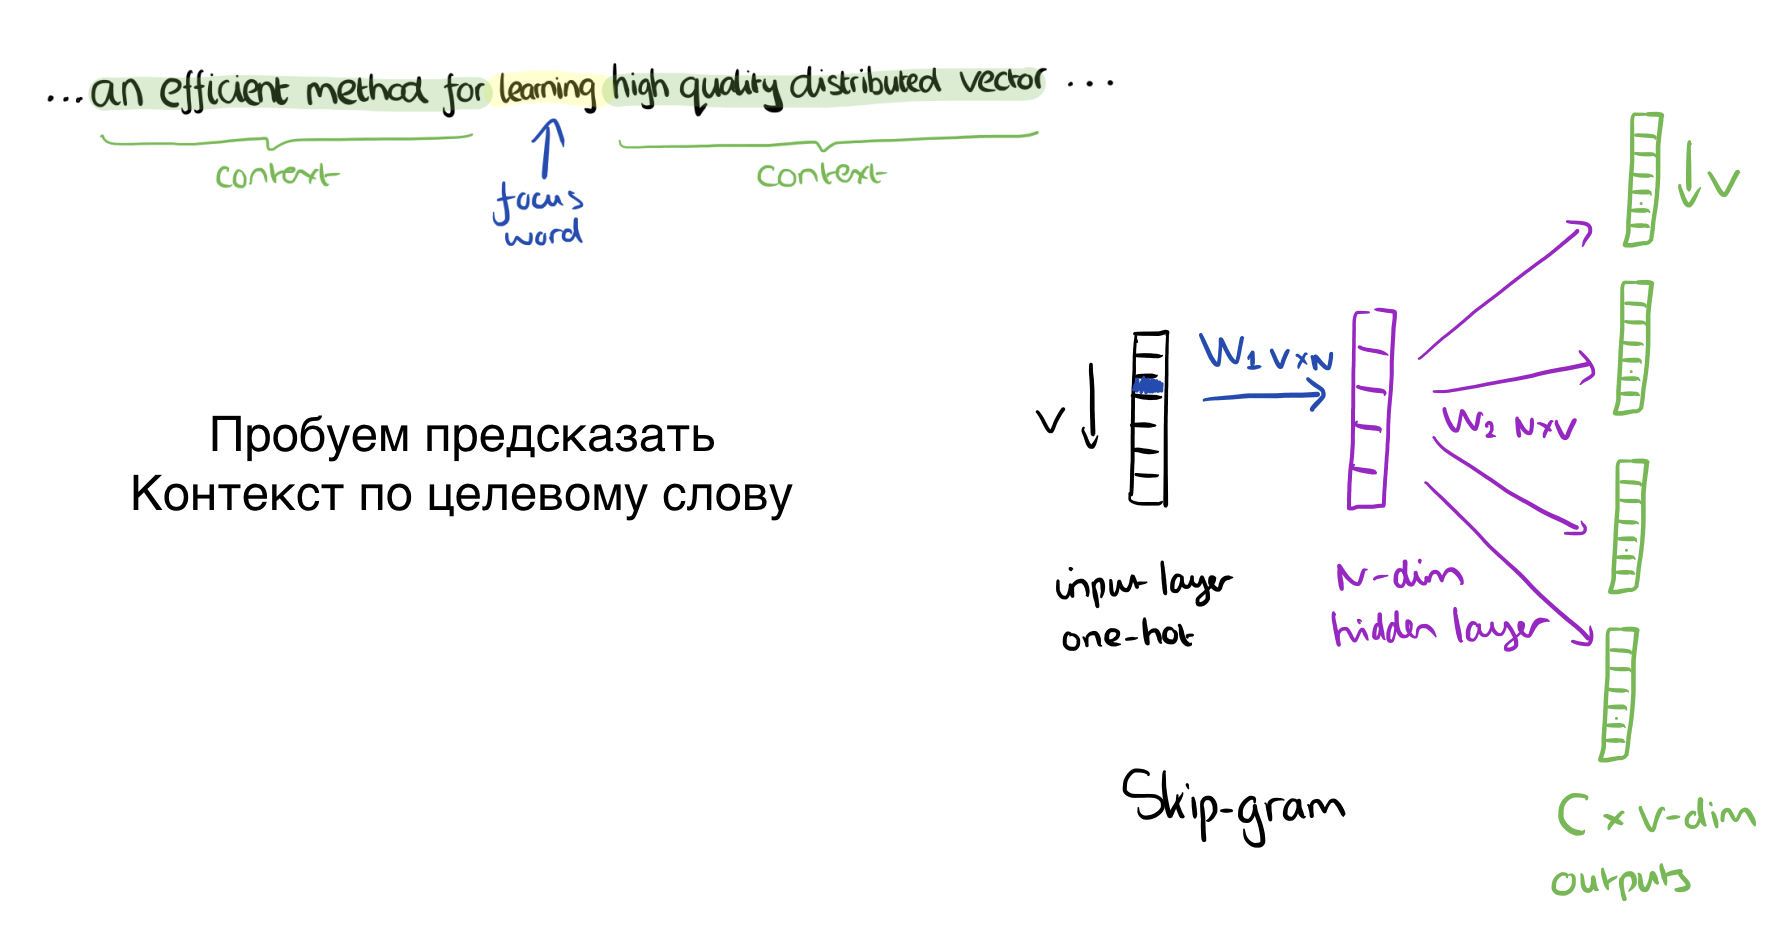
\includegraphics[width=.9\linewidth]{skipgram.png}
	\end{center}
	\vfill
	\footnotesize  {\color{blue} \url{https://blog.acolyer.org/2016/04/21/the-amazing-power-of-word-vectors/}}
\end{frame} 


\begin{frame}{CBOW}
\begin{center}
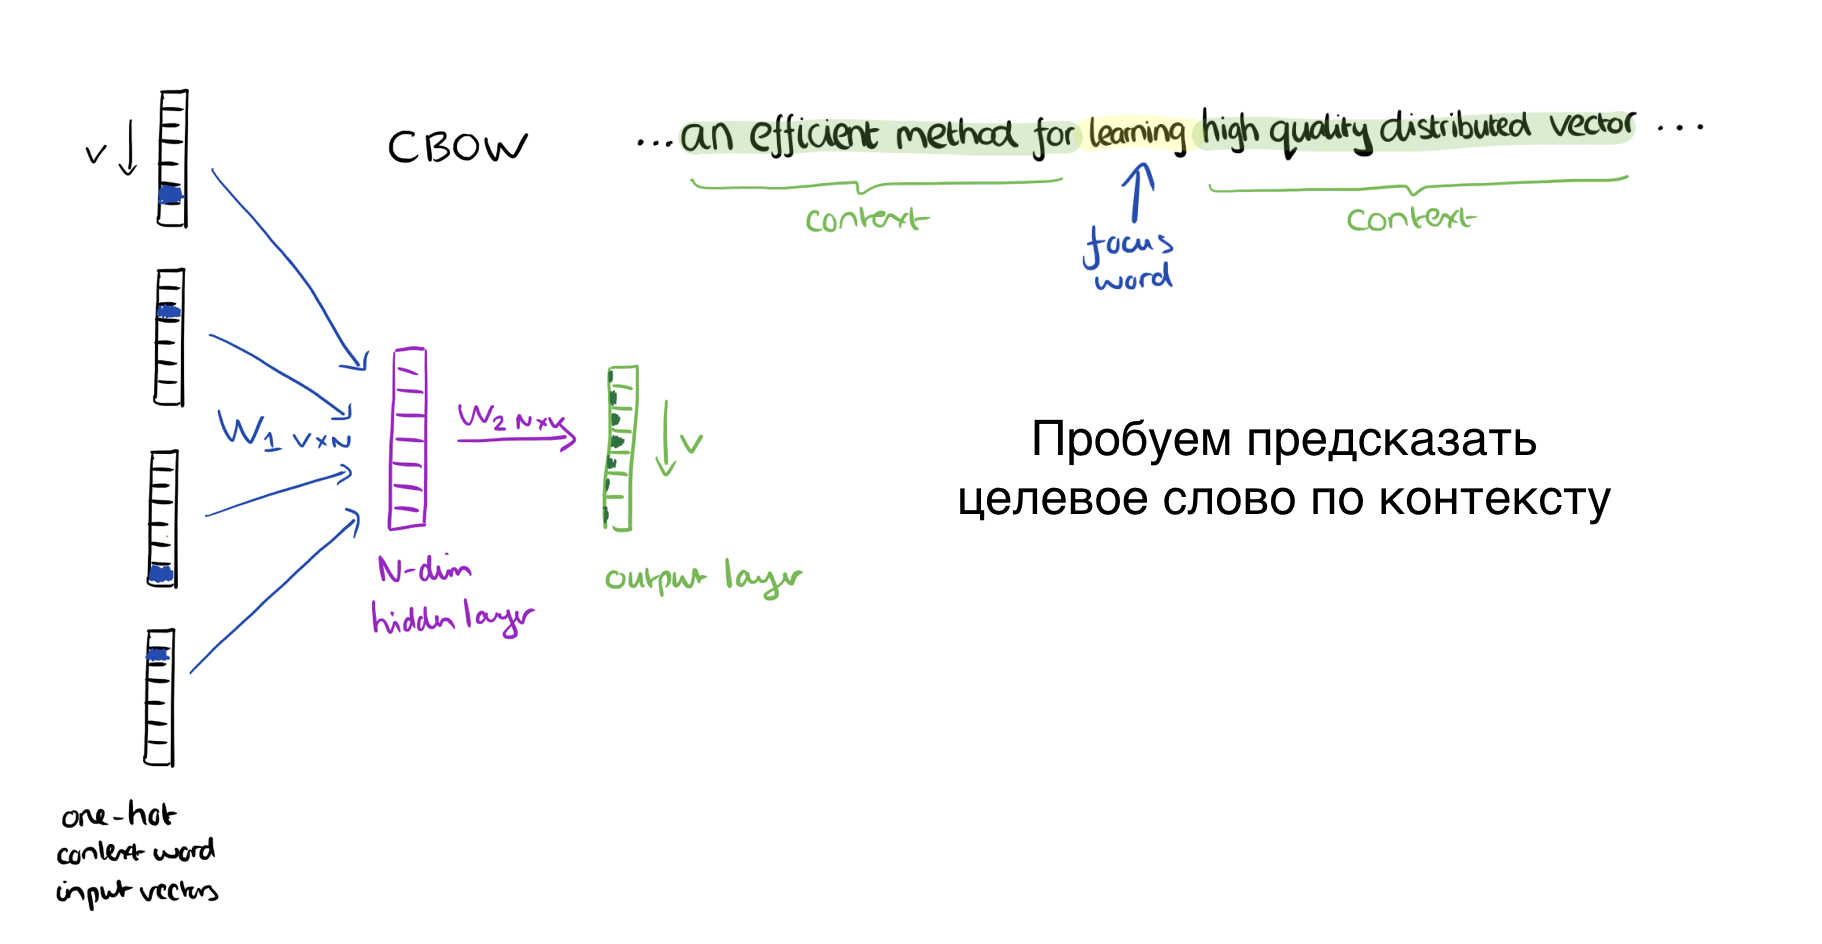
\includegraphics[width=.9\linewidth]{CBOW.png}
\end{center}
\vfill
\footnotesize  {\color{blue} \url{https://blog.acolyer.org/2016/04/21/the-amazing-power-of-word-vectors/}}
\end{frame} 


\begin{frame}{Гиперпараметры}
	\begin{wideitemize} 
			\item  Размер эмбединга (исторически $300$, но варианты $100, 500$ тоже возможно)
			
			\item  Число наблюдений для негативного сэмплирования (для маленьких датасетов $15-20,$ для больших $2-5$)
			
			\item  Окно контекста (обычно $5-10$), 
			
			\item  Очень большое окно —  похожесть топиков, можно вводить w2v через матричные разложения
		\end{wideitemize} 
\vfill
\footnotesize{\color{blue} \url{https://lena-voita.github.io/nlp_course/word_embeddings.html}}
\end{frame} 



\begin{frame}{Полезные мысли про обучение}
\begin{wideitemize} 
	\item В tensorflow довольно легко собрать свой собственный w2v и обучить его, но не стоит делать это.  Ваша реализация не будет такой эффективной, как уже существующие специализированные реализации. За последние годы алгоритмы для обучения w2v претерпели существенную эволюцию. 
	
	\item   Реализация w2v из пакета gensim зачастую работает быстрее, чем модели, написанные в стандартных для нейросеток бэкэндах. Это происходит из-за многопоточности и разных умных оптимизаций тонких мест в обучении. 
\end{wideitemize} 
\end{frame} 


\begin{frame}{Полезные мысли про обучение}
\begin{wideitemize} 
\item  При достаточно большом корпусе текстов можно не делать лемматизацию. Сетка сама поймёт по контексту, что слова близки и присвоит им похожие вектора.

\item Если у вас специфическая задача, в которой встречается специфическая лексика, возьмите предобученную на большом корпусе сетку и дообучите её под свои нужды.

\item \alert{w2v может выдавать эмбединги только для слов из заданного при обучении словоря.} Этот минус можно попытаться побороть и получить другую модель, fasttext
\end{wideitemize} 
\end{frame} 


\begin{frame}{Проблемы word2vec}
\begin{wideitemize} 
	\item Не умеем работать с новыми словами, которых не было в нашем словаре при обучении
	
	\item  Не закладываем никакой априорной информации о разных
	формах одного слова
	
	\item  Обучаемся на контекст слова, но всё ещё действуем в парадигме мешка слов, никак не учитываем порядок слов
	
	\item Не учитываем структуру слов, не умеем обрабатывать опечатки	
\end{wideitemize} 
\end{frame} 



\begin{transitionframe}
	\begin{center}
		\Huge  Как это использовать и где раздобыть?
	\end{center}
\end{transitionframe}


\begin{frame}{Как это использовать}
\begin{wideitemize} 
	\item Можно искать похожие слова
	
	\item  Можно менять формы слов
	
	\item  Можно искать определённые отношения
	
	\item  Можно использовать как признаки для моделей
	
	\item  Обучение w2v — аналог transfer learning, но обучение идёт на фиктивную задачу, разметка, сделанная вручную, не нужна
\end{wideitemize} 
\end{frame} 


\begin{frame}{Something2vec}
		\begin{wideitemize} 
			\item \alert{Эмбединги (embeddings)} — это сопоставление произвольной сущности (например, узла в графе или кусочка картинки) некоторому вектору.
			
			\item  Любую последовательность можно представить в виде эмбединга
			
			\item  Последовательность банковских транзакций
			
			\item  Веб-сессии (последовательность перехода по сайтам)
			
			\item Графы взаимосвязей между пользователями 
			
			\item Любая категориальная переменная: порядок, в котором турист посещал города; порядок, в котором юзер отранжировал сериалы и тп
		\end{wideitemize} 
\end{frame} 


\begin{frame}{something2vec}
	\begin{center}
		
\includegraphics[width=.8\linewidth]{smth2vec.png}
	\end{center}
\end{frame} 


\begin{frame}{Где взять уже готовое (Google)}
	\begin{center}
		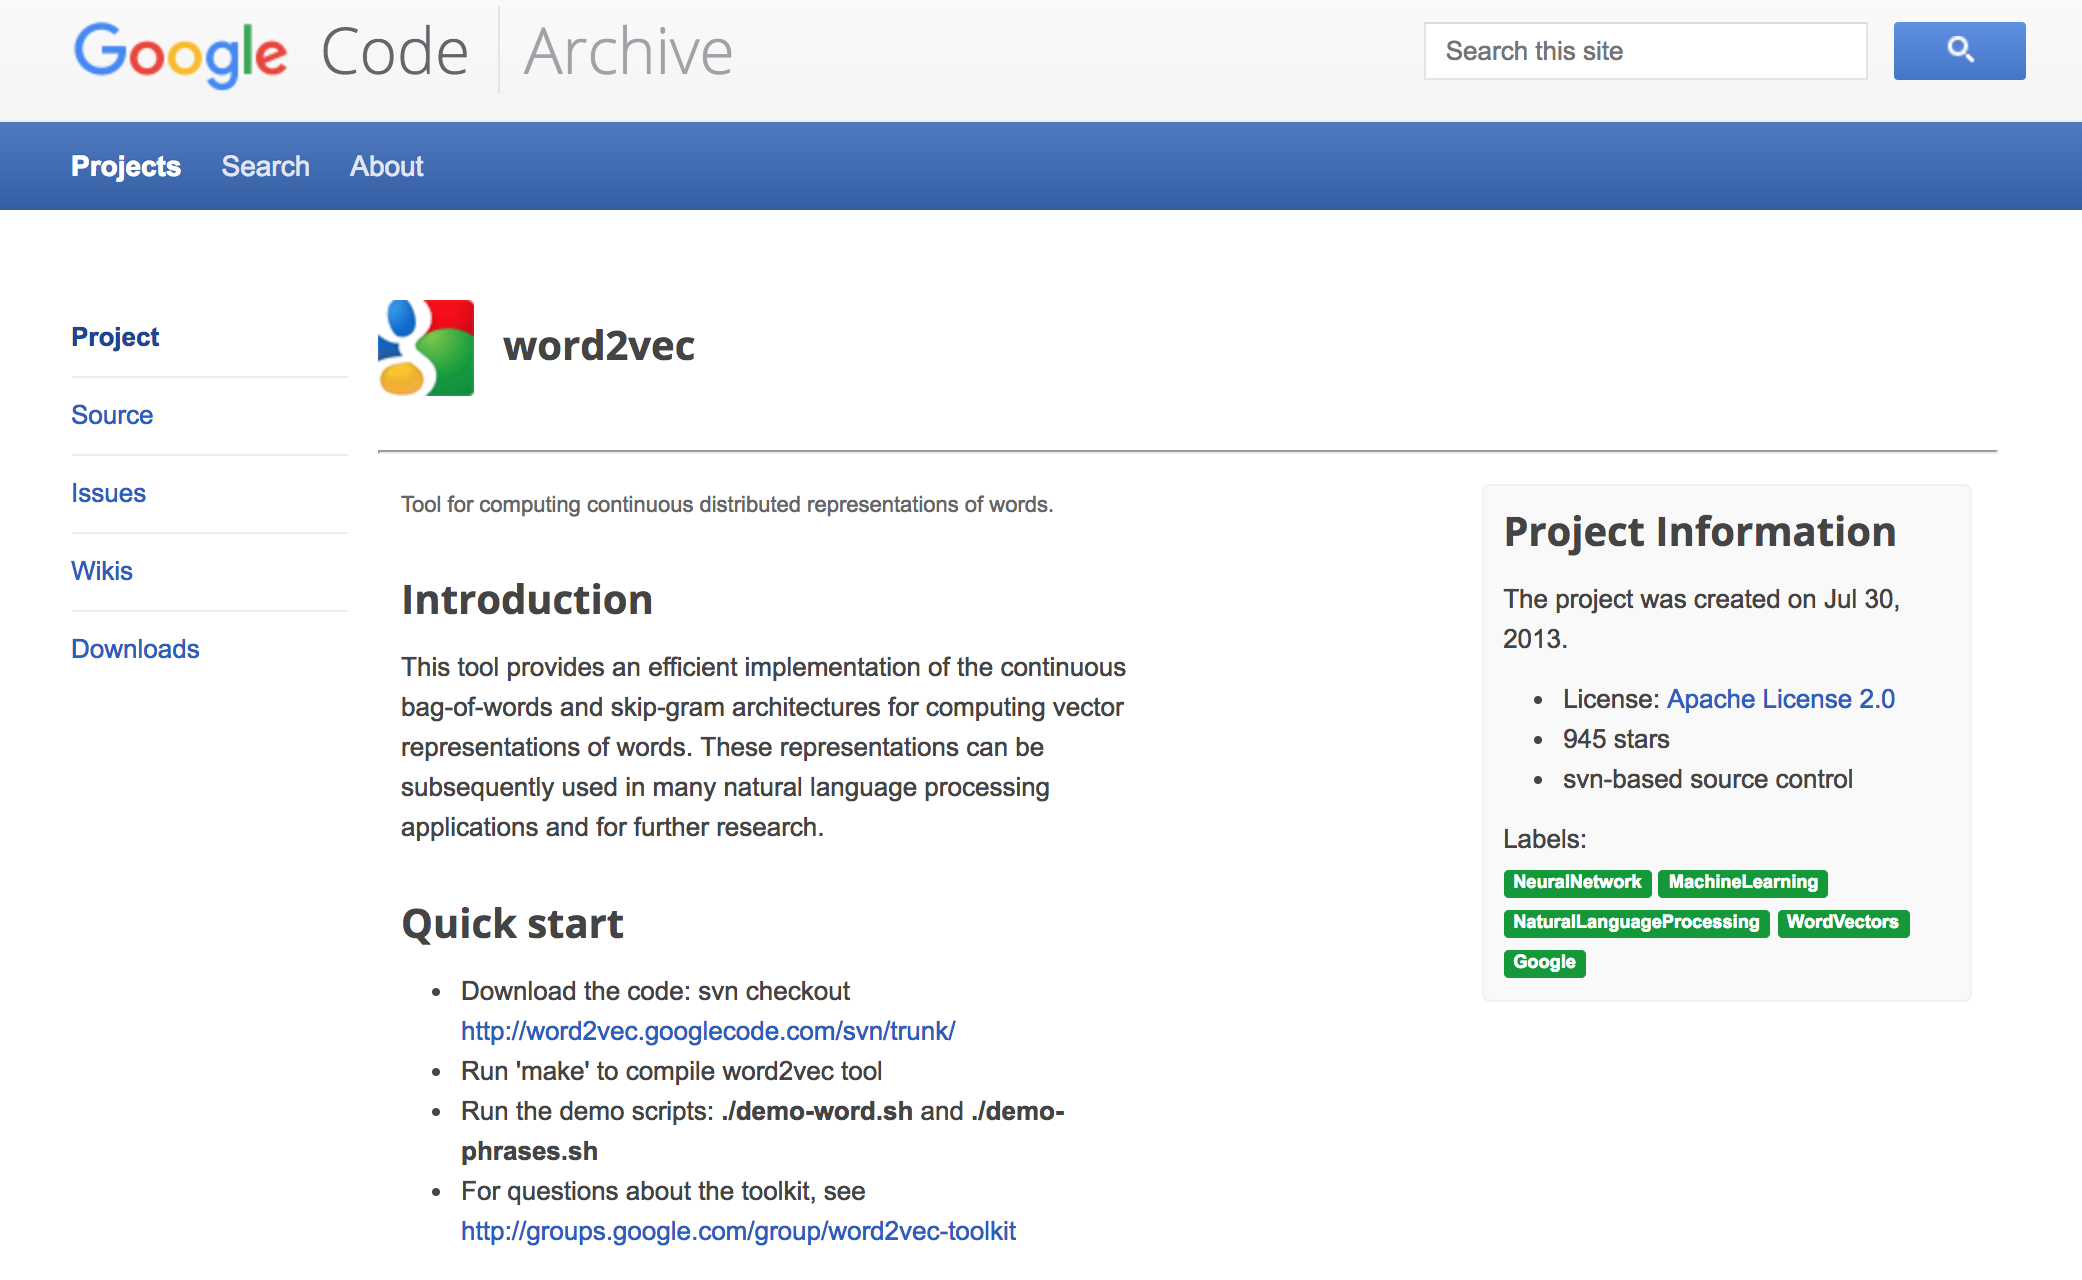
\includegraphics[width=.65\linewidth]{google_wv.png}
	\end{center}

	\vfill
	
	\footnotesize Гугловская модель для английского языка:  {\color{blue} \url{https://code.google.com/archive/p/word2vec/}}
\end{frame} 
	
	
\begin{frame}{Где взять уже готовое (проект RusVectōrēs)}
	\begin{center}
		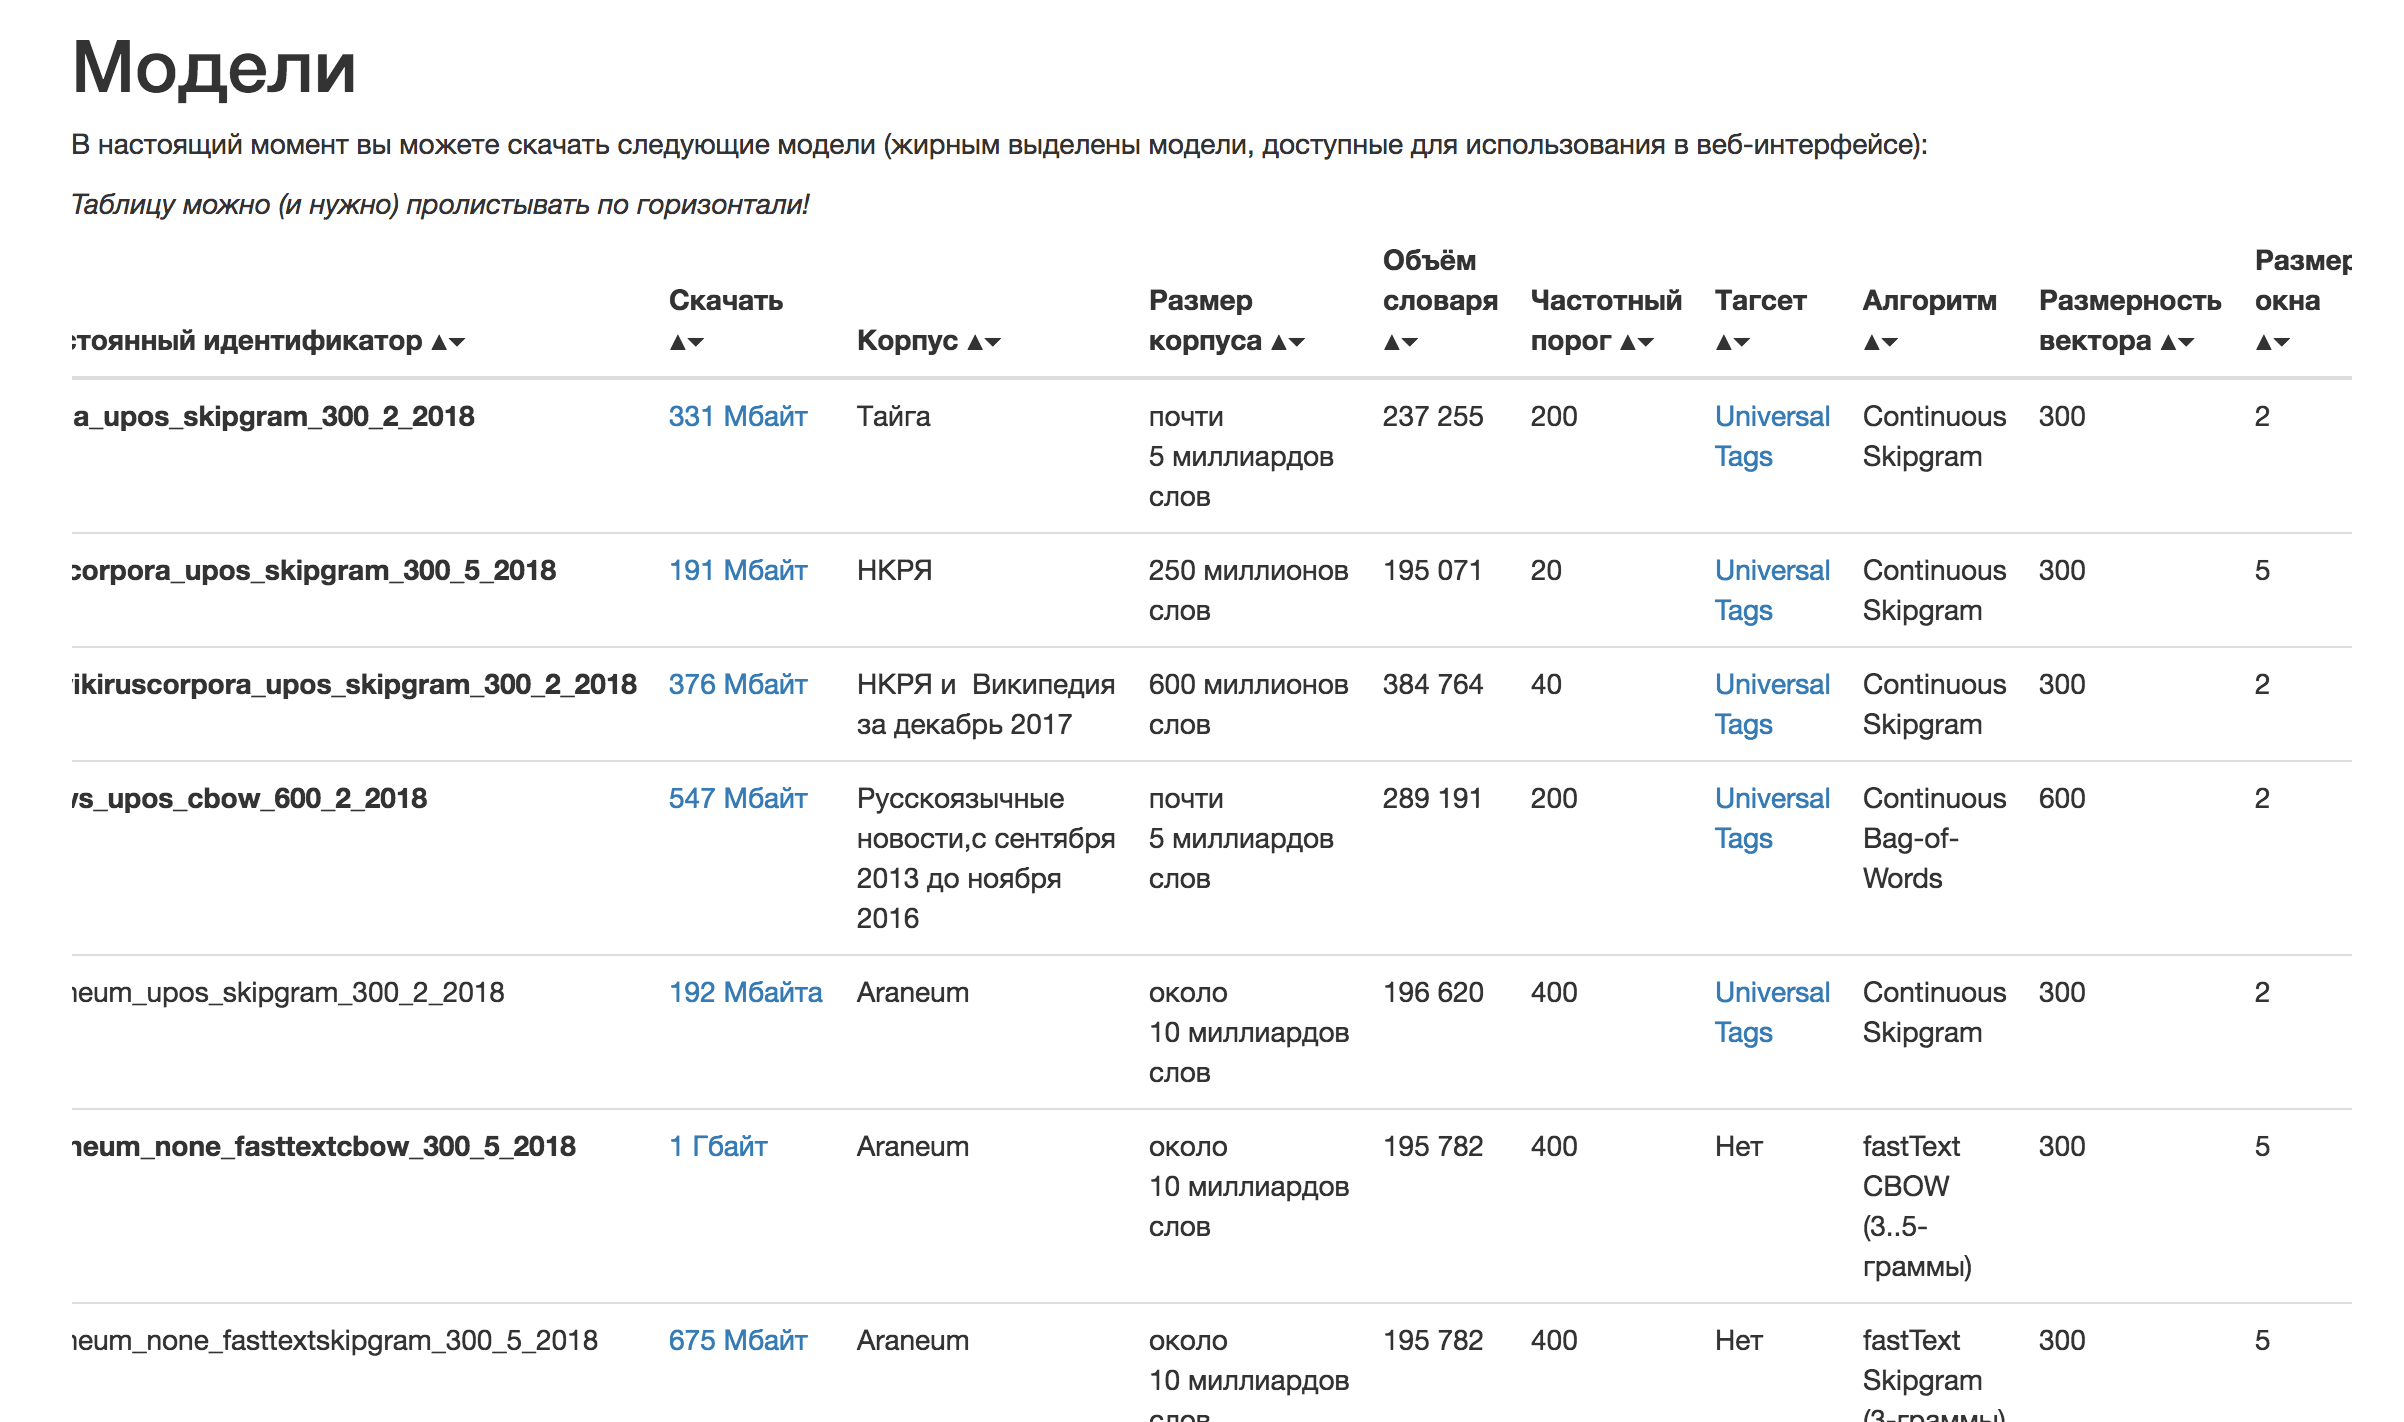
\includegraphics[width=.7\linewidth]{rusvec_models.png}
	\end{center}
	
		\vfill
	
		\footnotesize Куча разных моделей для русского языка:  {\color{blue} \url{https://rusvectores.org/ru/models/}}
\end{frame} 


\begin{frame}{Свойства word2vec}
	\begin{center}
		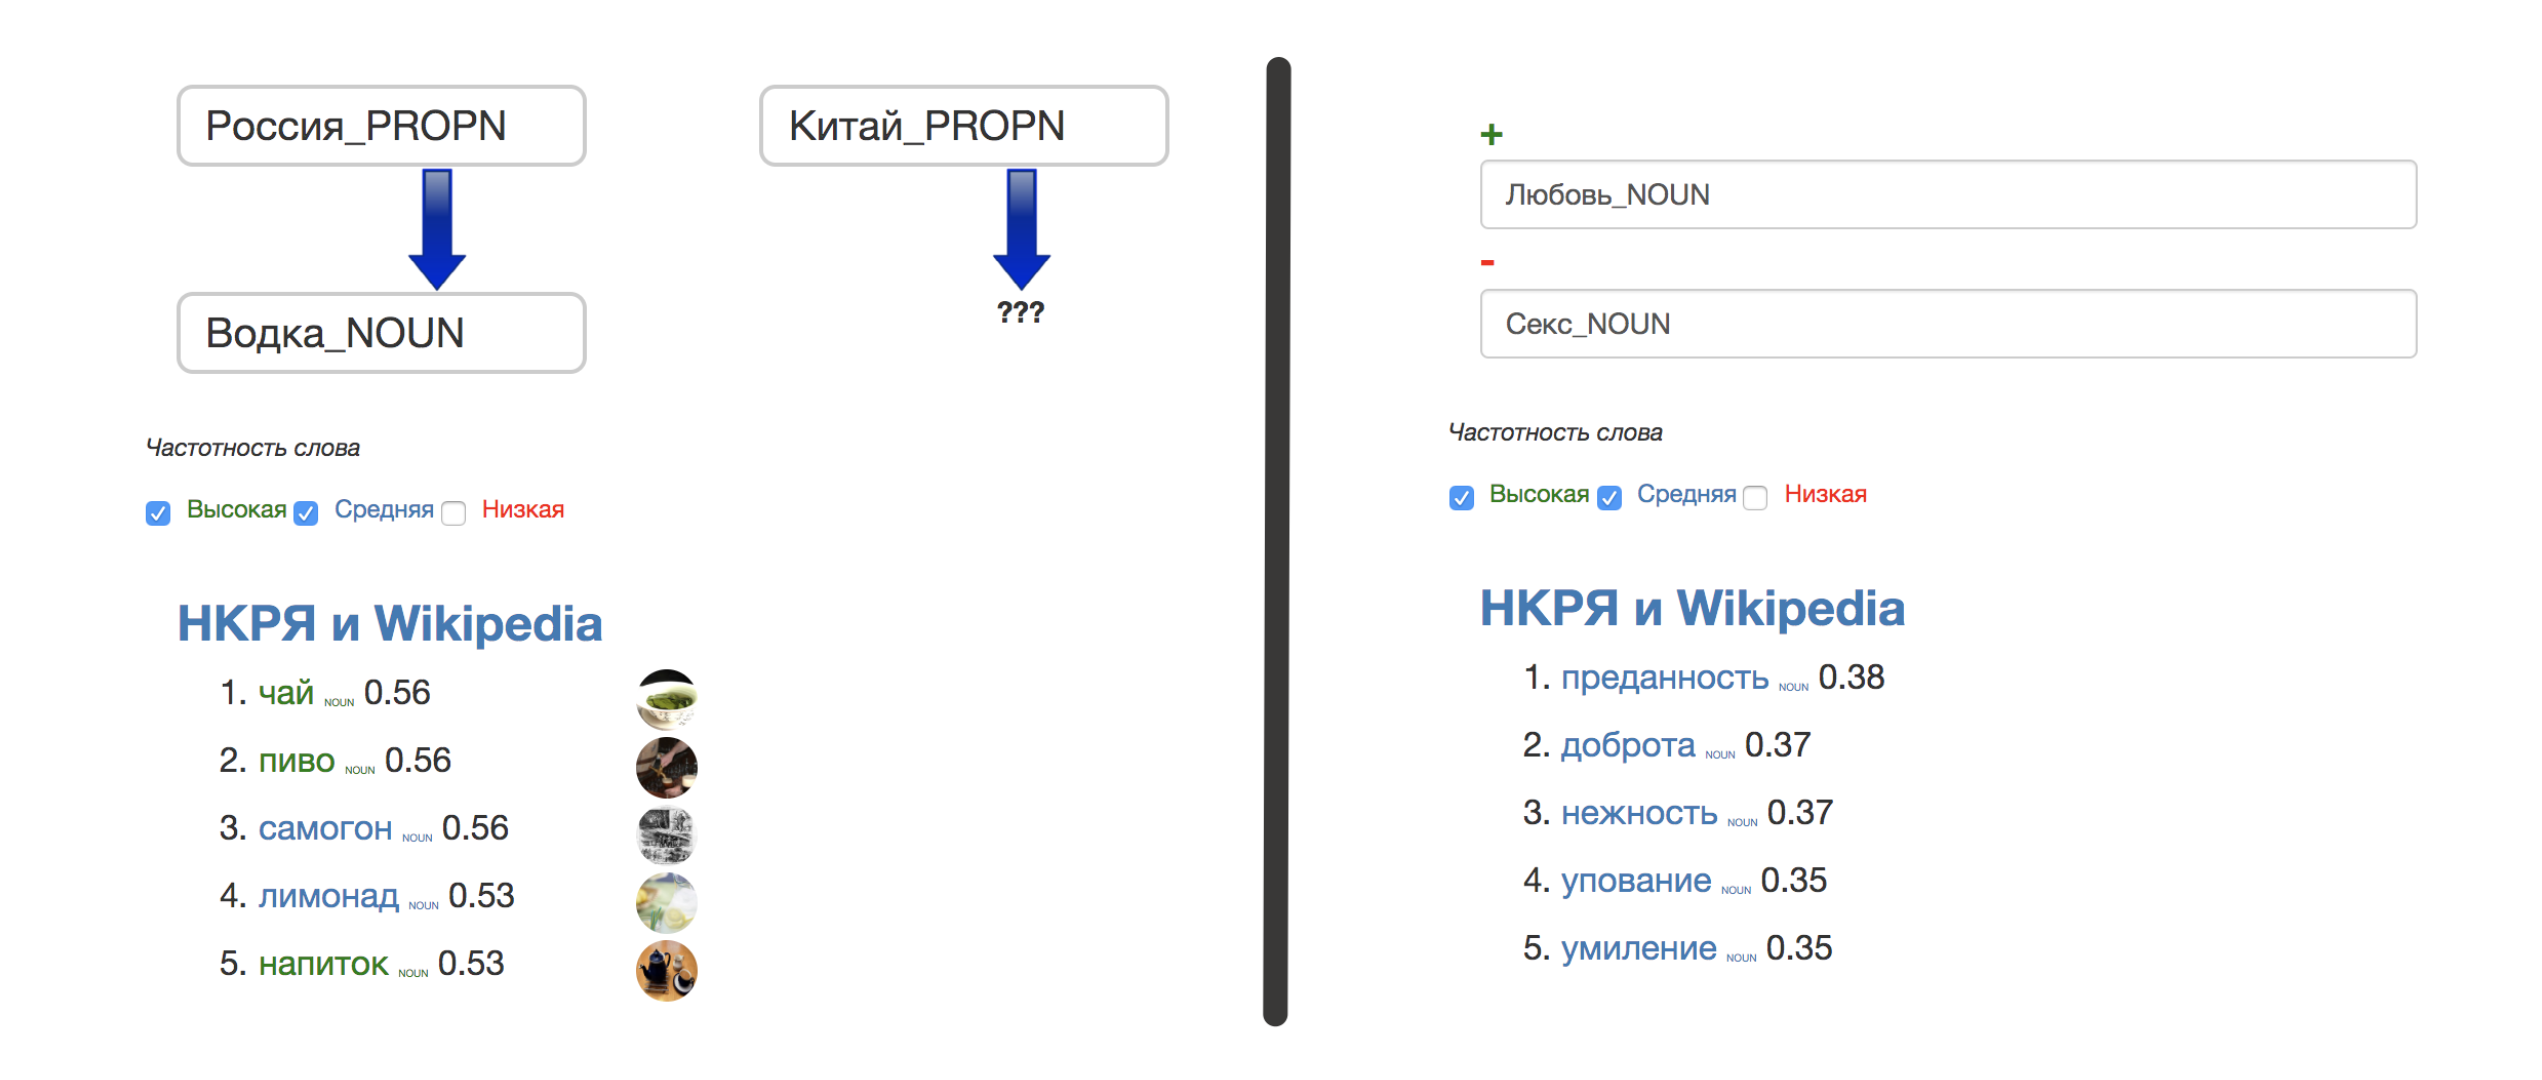
\includegraphics[width=.85\linewidth]{rusvec_calc2.png}
	\end{center}
	\vfill
	\footnotesize  {\color{blue} \url{https://rusvectores.org/ru/calculator}}
\end{frame} 


\begin{frame}{Свойства word2vec}
	Результат обучения векторных представлений сильно зависит от коллекции документов. \alert{Могут возникать неожиданные артефакты.}
	
	\begin{center}
		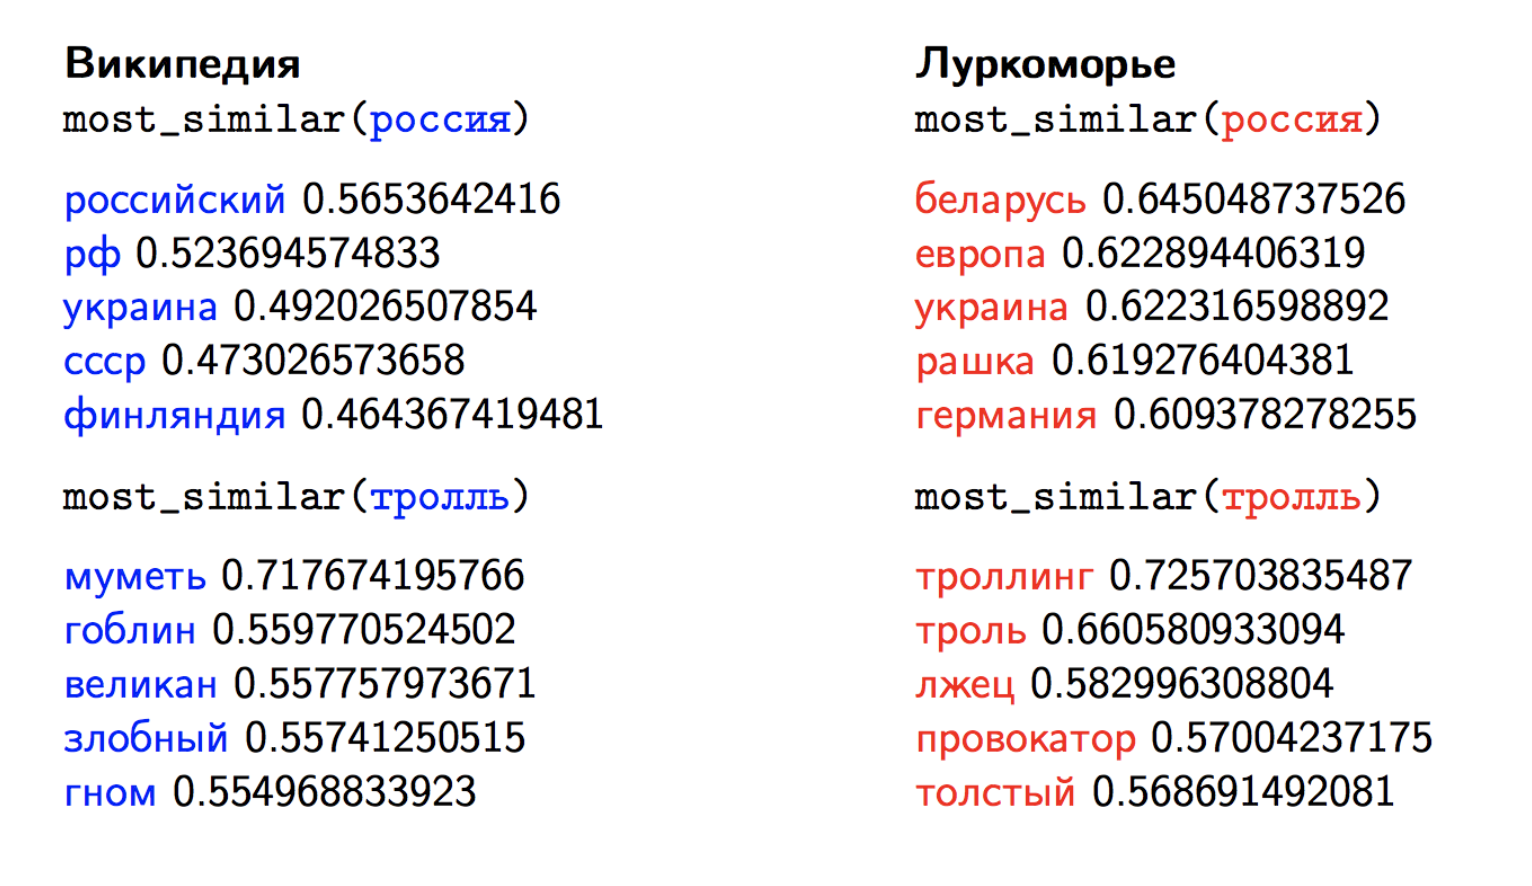
\includegraphics[width=.65\linewidth]{wikilurk.png}
	\end{center}
\end{frame} 


\begin{frame}{Модель - сексист}
	\begin{center}
		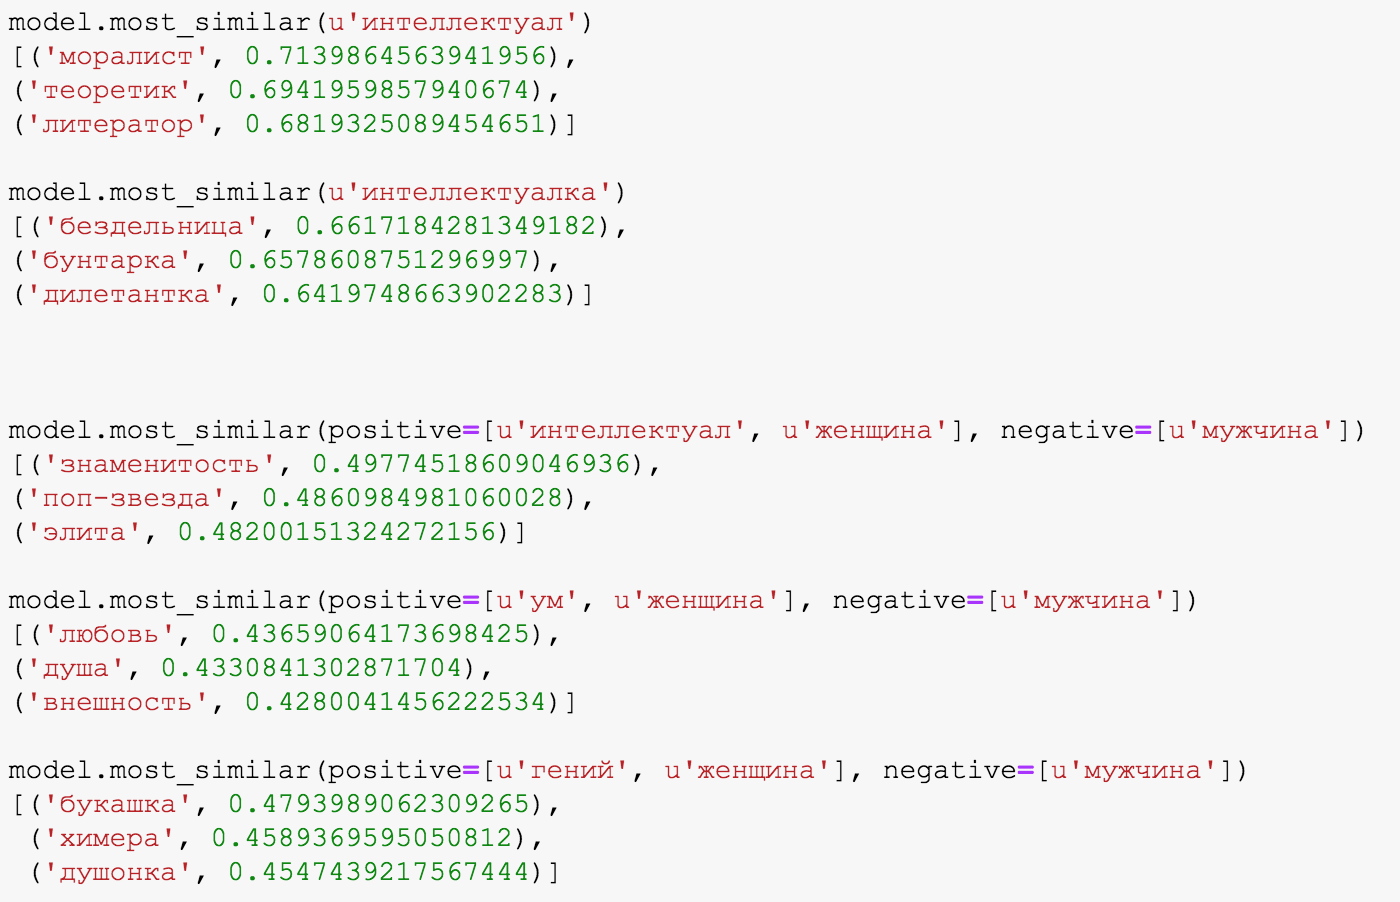
\includegraphics[width=.65\linewidth]{w2v_sex.png}
	\end{center}
	\vfill
	\footnotesize  {\color{blue} \url{https://nikolenko.livejournal.com/267442.html}}
\end{frame} 


\begin{frame}{Word2vec всего лишь модель}
	\begin{center}
		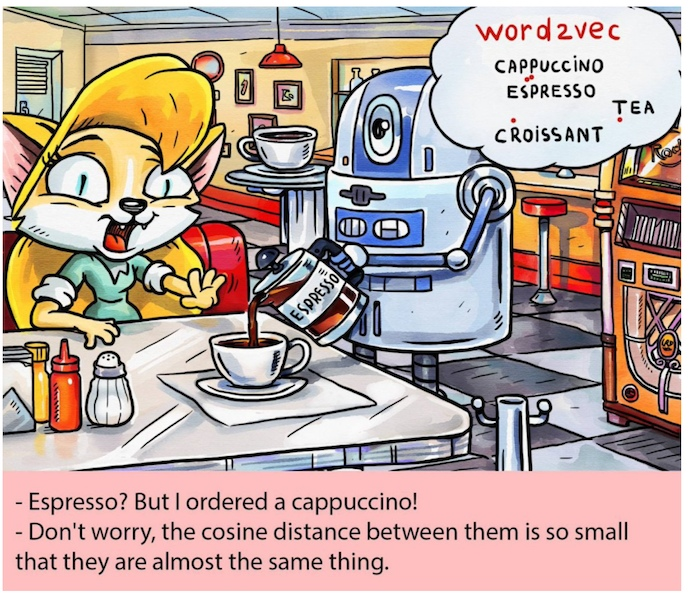
\includegraphics[width=.55\linewidth]{w2v_idiot.jpg}
	\end{center}
\end{frame} 


\begin{frame}{Откуда взять данные (дампы Википедии)}
	\begin{center}
		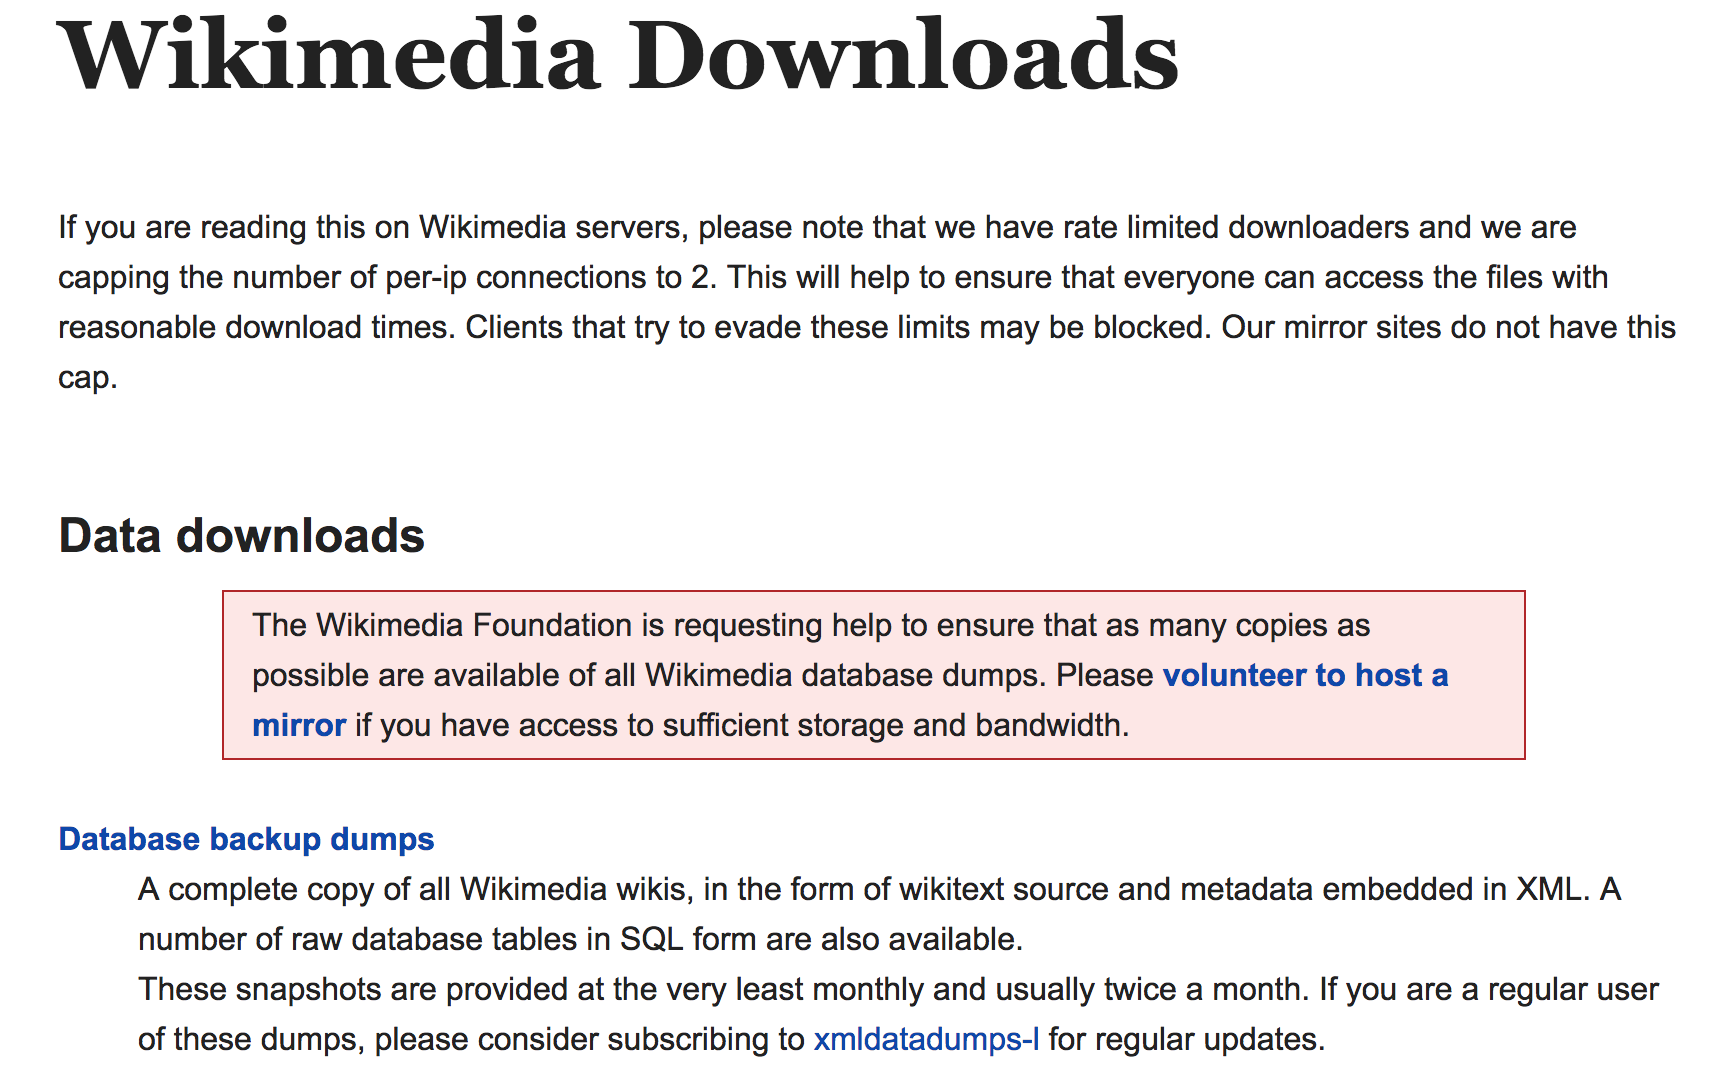
\includegraphics[width=.7\linewidth]{wiki_dumps.png}
	\end{center}
	
	\vfill
	
	\footnotesize Дампы википедии для разных языков:  {\color{blue} \url{https://dumps.wikimedia.org}} \newline Например, для русского:  {\color{blue} \url{https://dumps.wikimedia.org/ruwiki/}} 
\end{frame} 


\begin{frame}{Откуда взять данные (НКРЯ)}
	\begin{center}
	
\includegraphics[width=.99\linewidth]{ruscorp.png}
	\end{center}
	
	\vfill
	
	\footnotesize Национальный корпус Русского языка:  {\color{blue} \url{http://ruscorpora.ru}} 
\end{frame} 



\begin{transitionframe}
	\begin{center}
		\Huge  Классификация текстов
	\end{center}
	\centering 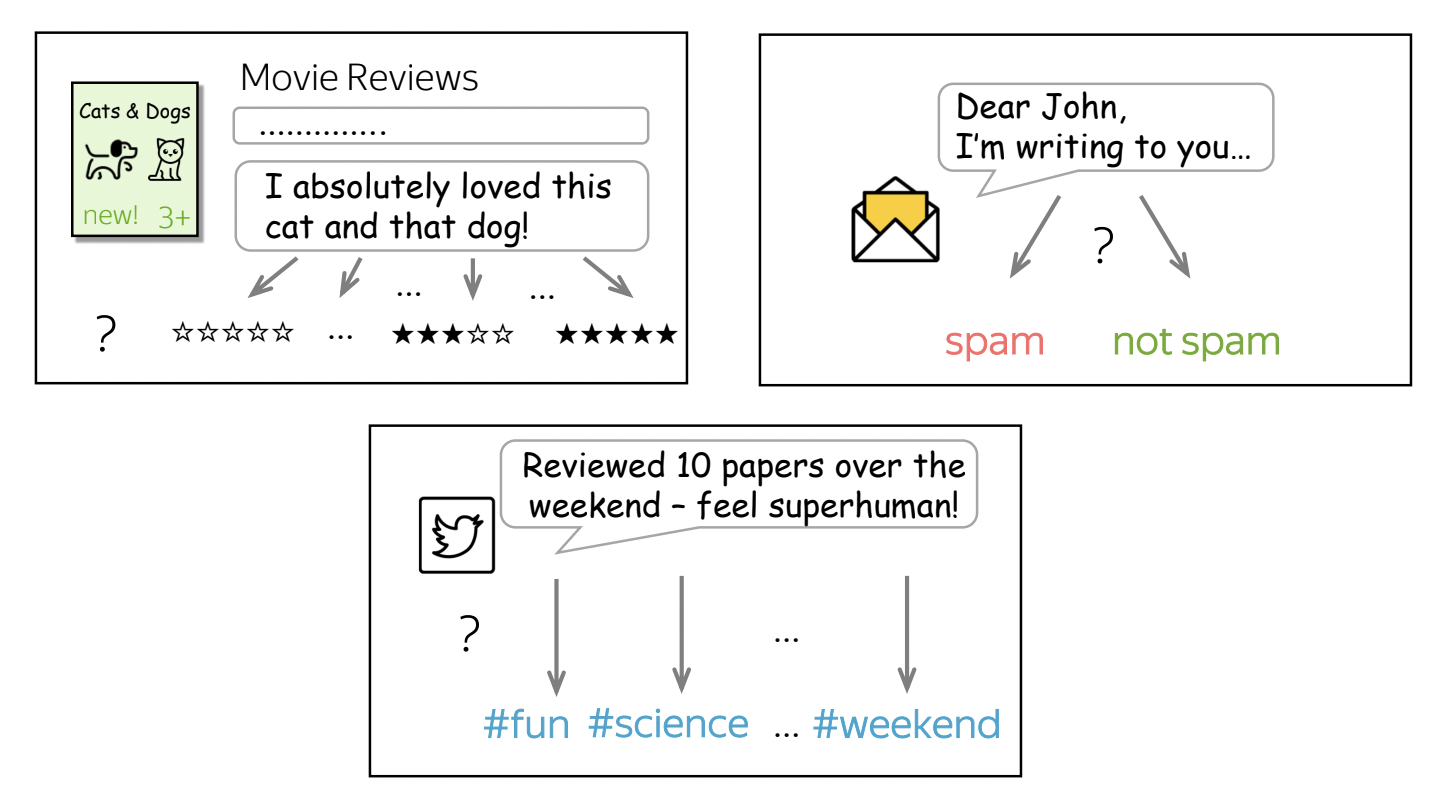
\includegraphics[width=.6\linewidth]{clf_ex.png}
\end{transitionframe}


\begin{frame}{Классификация текстов}
	\begin{center}
		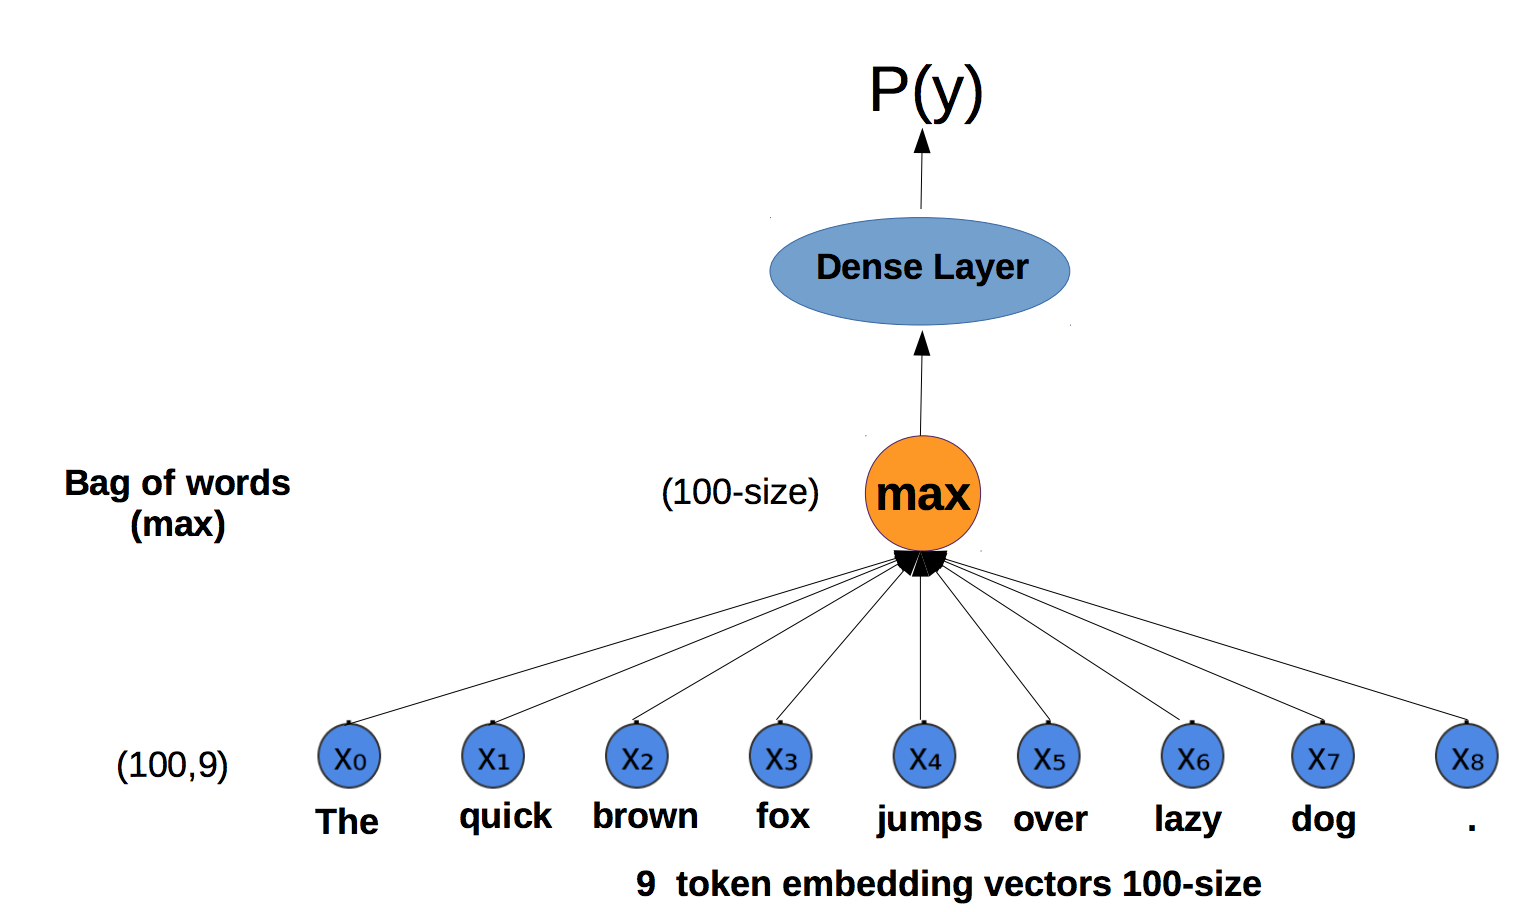
\includegraphics[width=.75\linewidth]{text_nn.png}
	\end{center}
\end{frame} 


\begin{frame}{Проблемы}
	\begin{wideitemize} 
		\item  Теряем информацию о порядке слов 
		\item  Очень бедно используем информацию из эмеддингов
		\item  \alert{Давайте учить нейросеть!}
	\end{wideitemize} 
\end{frame} 


\begin{frame}{Классификация текстов}
	\begin{center}
		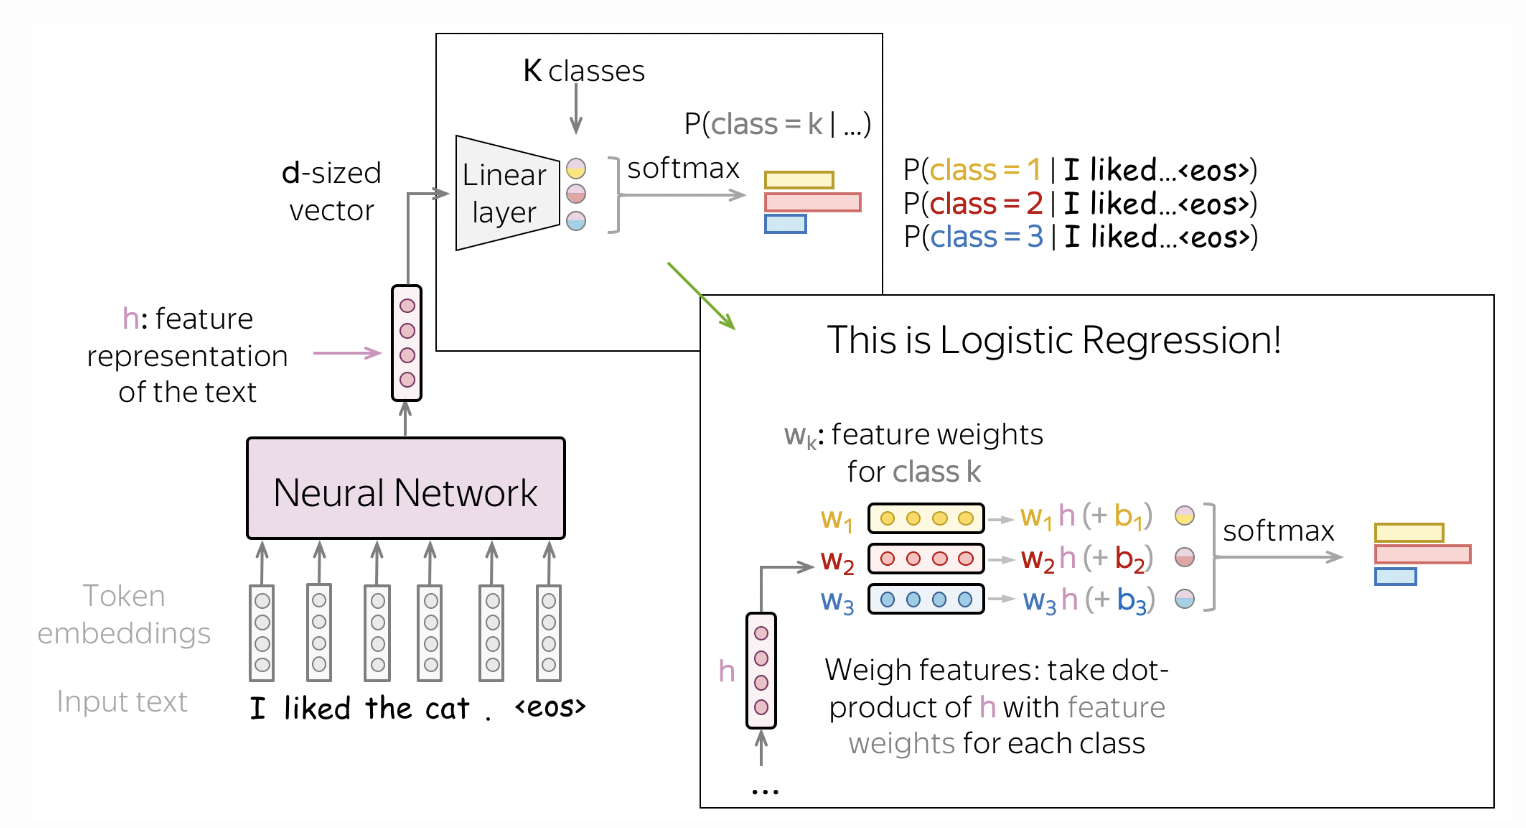
\includegraphics[width=.85\linewidth]{clf_pipe.png}
	\end{center}
	
	\vfill
	\footnotesize  {\color{blue} \url{https://lena-voita.github.io/nlp_course/text_classification.html}} 
\end{frame} 


\begin{frame}{Классификация текстов (RNN)}
	\begin{center}
		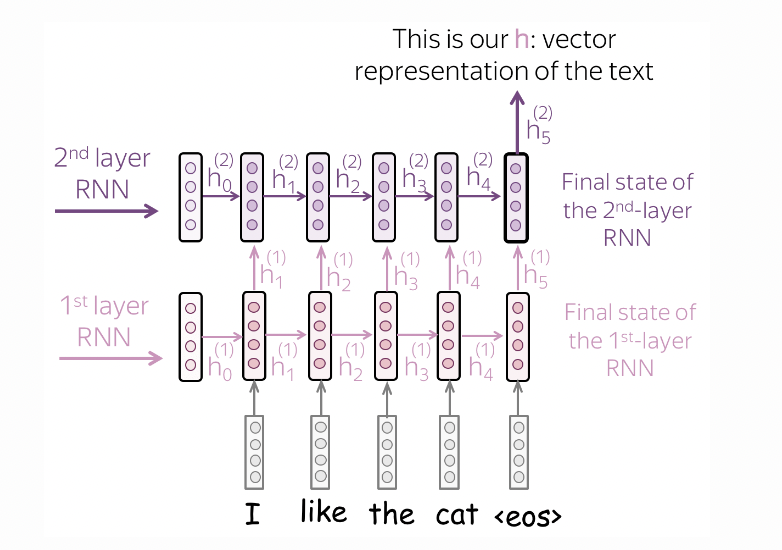
\includegraphics[width=.65\linewidth]{rnn_clf.png}
	\end{center}
	
	\vfill
	\footnotesize  {\color{blue} \url{https://lena-voita.github.io/nlp_course/text_classification.html}} 
\end{frame} 


\begin{frame}{Классификация текстов (Bidirectional RNN)}
	\begin{center}
		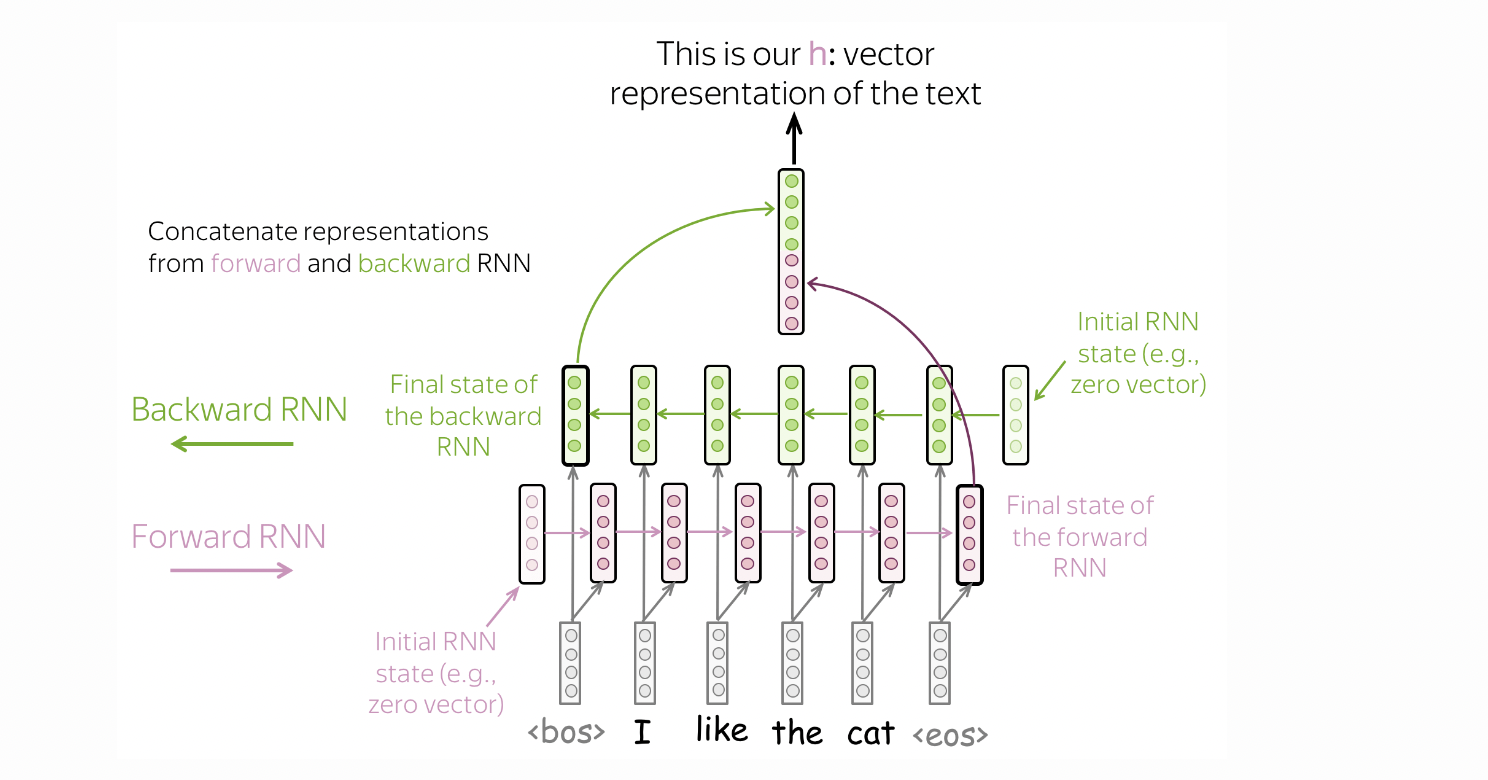
\includegraphics[width=.85\linewidth]{bidir_clf.png}
	\end{center}
	
	\vfill
	\footnotesize  {\color{blue} \url{https://lena-voita.github.io/nlp_course/text_classification.html}} 
\end{frame} 


\begin{frame}{Классификация текстов (СNN)}
	\begin{center}
		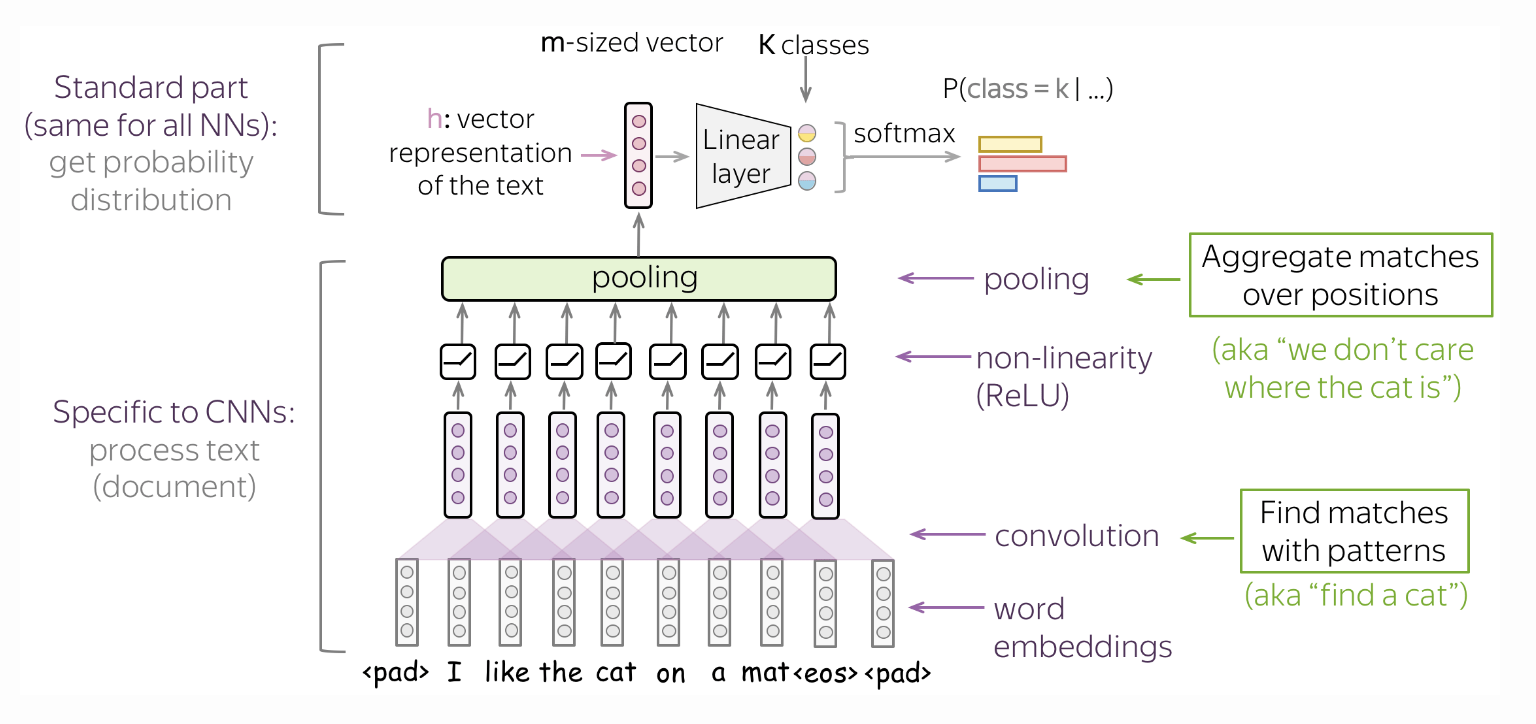
\includegraphics[width=.85\linewidth]{cnn_clf_t.png}
	\end{center}
	
	\vfill
	\footnotesize  {\color{blue} \url{https://lena-voita.github.io/nlp_course/text_classification.html}} 
\end{frame} 


\begin{frame}{1D свёртка}
\begin{center}
	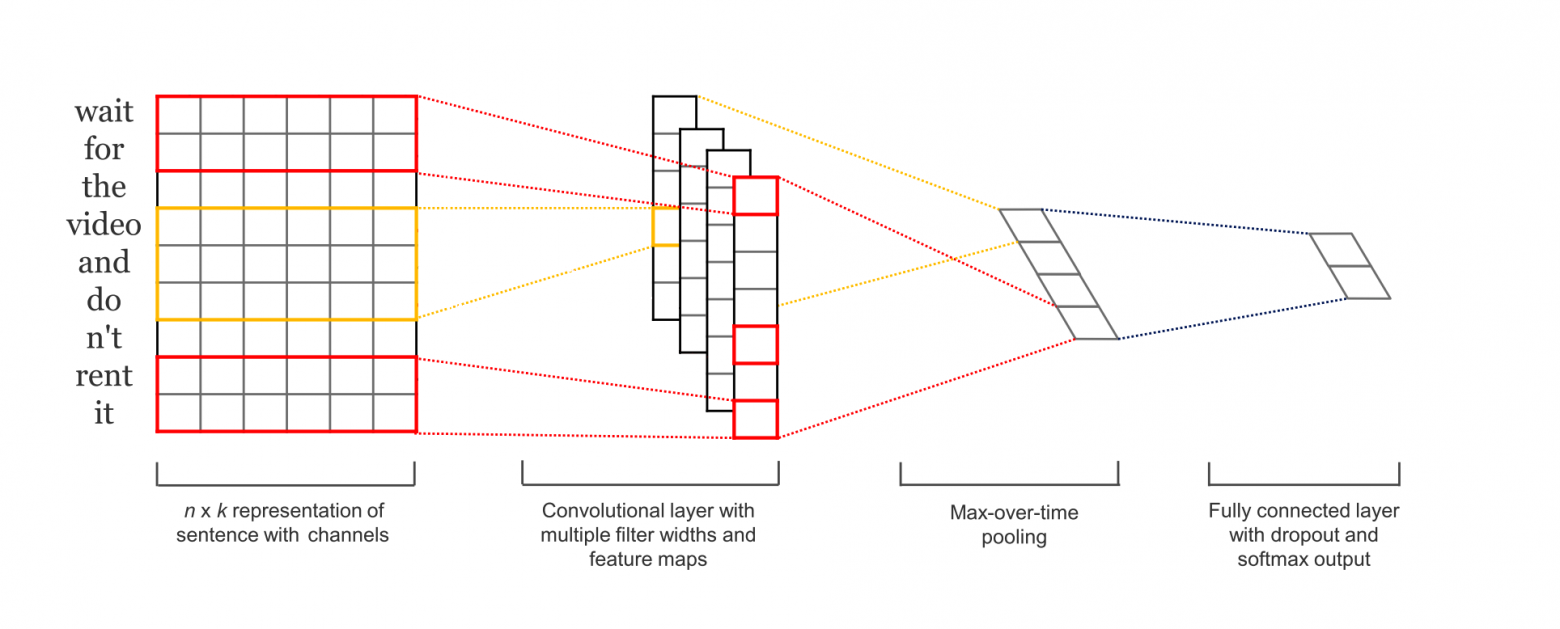
\includegraphics[width=.99\linewidth]{1d_conv.png}
\end{center}
\end{frame} 


\begin{frame}{Резюме}
	\begin{wideitemize} 
		\item  Поверх эмбеддингов можно собрать любую архитектуру
		\item  Эмбеддинги можно учить одновременно с классификатором
		\item  Можно обучить эмбеддинги на большом корпусе текстов и доучить под конкретный классификатор
		\item  Можно обучать эмбеддинги более сложными способами \alert{$\Rightarrow$ автокодировщики}
	\end{wideitemize} 
\end{frame} 

\end{document}



